\documentclass[12pt,a4paper]{article}
\usepackage[utf8]{inputenc}
\usepackage[german]{babel}
\usepackage[T1]{fontenc}
\usepackage{amsmath}
\usepackage{amsfonts}
\usepackage{amssymb}
\usepackage{graphicx}
\usepackage{array}
\usepackage[hidelinks]{hyperref}

%Schrift
\usepackage{newtxtext,newtxmath} 

% Literatur: eindeutige Autor-Jahr-Kürzel gemäß FTK-Leitfaden.
% natbib=true erhält die vorhandenen \citep-Befehle und ihre Seitenangaben.
\usepackage{csquotes}
\usepackage[backend=biber,style=alphabetic,sorting=nyt,natbib=true]{biblatex}
\usepackage{xurl}
\addbibresource{literatur.bib}

% Führende Artikel nur für die Kürzelbildung bei geklammerten Institutionsnamen
% entfernen; vollständige Autorenangaben und explizite shortauthor-Werte erhalten.
\DeclareSourcemap{
    \maps[datatype=bibtex]{
        \map{
            \step[notfield=shortauthor,final]
            \step[fieldsource=author,match=\regexp{\A\{(?:The|A|An|Der|Die|Das)\s+},final]
            \step[fieldset=shortauthor,origfieldval]
            \step[fieldsource=shortauthor,match=\regexp{\A(\{)(?:The|A|An|Der|Die|Das)\s+},replace=\regexp{$1}]
        }
    }
}

\usepackage[left=4cm,right=2cm,top=3cm,bottom=3cm,footskip=1.75cm]{geometry}

% FTK-Layout: einzeiliger Text mit einer Leerzeile zwischen Absätzen.
\usepackage[skip=\baselineskip,indent=0pt]{parskip}
\usepackage{titlesec}
\titleformat{\section}{\normalfont\raggedright\fontsize{16}{19.2}\selectfont\bfseries}{\thesection}{1em}{}
\titleformat{\subsection}{\normalfont\raggedright\fontsize{14}{16.8}\selectfont\bfseries}{\thesubsection}{1em}{}
\titleformat{\subsubsection}{\normalfont\raggedright\fontsize{12}{14.4}\selectfont\bfseries}{\thesubsubsection}{1em}{}
\titleformat{\paragraph}[block]{\normalfont\raggedright\fontsize{12}{14.4}\selectfont\itshape}{\theparagraph}{1em}{}
\titlespacing*{\section}{0pt}{0pt}{\baselineskip}
\titlespacing*{\subsection}{0pt}{2\baselineskip}{\baselineskip}
\titlespacing*{\subsubsection}{0pt}{2\baselineskip}{\baselineskip}
\titlespacing*{\paragraph}{0pt}{2\baselineskip}{\baselineskip}

% Tabellen und Beschriftungen einheitlich in 10 pt.
\usepackage{etoolbox}
\AtBeginEnvironment{tabular}{\fontsize{10}{12}\selectfont}
\usepackage{caption}
\DeclareCaptionFont{ftk}{\fontsize{10}{12}\selectfont}
\captionsetup{font=ftk,format=hang,justification=raggedright,singlelinecheck=false}
\captionsetup[table]{position=top}
\captionsetup[figure]{position=bottom}

% Seitenzahl rechts unten; Grundschrift der Fußzeile 10 pt, Seitenzahl 12 pt.
\usepackage{fancyhdr}
\fancypagestyle{ftk}{
    \fancyhf{}
    \fancyfoot[R]{\normalfont\fontsize{10}{12}\selectfont{\fontsize{12}{14.4}\selectfont\thepage}}
    \renewcommand{\headrulewidth}{0pt}
    \renewcommand{\footrulewidth}{0.4pt}
}
\pagestyle{ftk}
\setlength{\emergencystretch}{3em}
\author{Christian Koch}

\title{Bachelorthesis\\Attribute Stream-Based Access Control im Linux-Kernel}
\begin{document}
\hypersetup{pageanchor=false}
\pagenumbering{gobble}
\maketitle
\thispagestyle{empty}

\clearpage
\pagenumbering{roman}
\hypersetup{pageanchor=true}

\tableofcontents

\clearpage
\pagenumbering{arabic}

\section{Einleitung}

\subsection{Motivation}
Die Sicherheit von Linux-Systemen ist ein fundamentales Anliegen in der heutigen IT-Landschaft. 
Das Linux Security Module Framework stellt Schnittstellen bereit, über die Sicherheitsmodule unterschiedliche Zugriffskontrollmodelle im Linux-Kernel durchsetzen können\citep{kernelorgLSM}.
LSM-Hooks ermöglichen es, sicherheitsrelevante Kerneloperationen abzufangen und auf dieser Grundlage Zugriffsentscheidungen zu treffen.
Ein LSM-Hook prüft einen Zugriff jedoch grundsätzlich zu dem Zeitpunkt, an dem die jeweilige Kerneloperation ausgeführt wird.
Bei dauerhaft bestehenden Zugriffen wird eine spätere Änderung der Entscheidungsgrundlage dadurch nicht automatisch erneut bewertet.



\subsection{Wissenschaftliche Fragestellung}
Diese Arbeit untersucht, wie zentrale Prinzipien von Attribute Stream-Based Access Control für Dateiöffnungen unter Linux prototypisch umgesetzt werden können.
Im Mittelpunkt steht dabei die Frage, wie dynamische Attribute aus dem Userspace für Zugriffsentscheidungen eines eBPF-LSM-Programms bereitgestellt und Änderungen bei bereits bestehenden Dateizugriffen nachträglich berücksichtigt werden können.

Daraus ergibt sich folgende wissenschaftliche Fragestellung:

\begin{quote}
Wie kann Attribute Stream-Based Access Control für Dateiöffnungen prototypisch mittels eBPF-LSM unter Linux umgesetzt werden, und welche technischen Einschränkungen ergeben sich insbesondere bei der nachträglichen Kontrolle bereits bestehender Dateizugriffe?
\end{quote}

Zur Beantwortung dieser Fragestellung werden insbesondere die Überführung textueller Policy-Dateien in eine kernelgeeignete Repräsentation, die Bereitstellung dynamischer Attribute für Zugriffsentscheidungen im Kernel sowie die nachträgliche Überwachung bestehender Zugriffssituationen betrachtet.

\subsection{Zielsetzung}
Zielsetzung der Arbeit ist ein Prototyp, der zentrale Eigenschaften von Attribute Stream-Based Access Control auf die Kontrolle von Dateiöffnungen unter Linux überträgt.
Insbesondere sollen Stream-Attribute wie Zeitinformationen sowie externe, zur Laufzeit aktualisierte Attribute in die Zugriffsentscheidung einbezogen werden.
Der Prototyp soll textuelle Policies einlesen, in eine kernelgeeignete Repräsentation übersetzen und neue Dateiöffnungen mittels eBPF-LSM im Kernel bewerten.
Nach der erfolgreichen Aktivierung geänderter Policies oder Attribute sowie beim Erreichen entscheidungsrelevanter Zeitgrenzen soll er bereits bestehende Dateizugriffe im Userspace ereignisbasiert erneut bewerten und bei einer festgestellten Verletzung einen Entzug versuchen.

Nicht Gegenstand der Arbeit ist die vollständige Implementierung der Publish-Subscribe-Architektur der Streaming Attribute Policy Language oder eines allgemeinen, eigenständigen ASBAC-PDP.
Der Prototyp ist auf Dateiöffnungen über den LSM-Hook \texttt{file\_open} und auf die nachträgliche Untersuchung geöffneter File Descriptors beschränkt.


\subsection{Aufbau der Arbeit}
Kapitel~2 führt die für die Arbeit erforderlichen Grundlagen ein. Dazu gehören der Reference-Monitor-Ansatz, Attribute-Based Access Control und Attribute Stream-Based Access Control sowie die für die Umsetzung relevanten Linux-Technologien LSM, eBPF und eBPF-Maps. Zudem wird der eigene Ansatz gegenüber der Publish-Subscribe-Architektur von SAPL und verwandten Konzepten fortdauernder Autorisierung abgegrenzt.

Kapitel~3 leitet aus der Zielsetzung die funktionalen, operativen und entwicklungsbezogenen Anforderungen an den Prototyp ab. Kapitel~4 entwickelt darauf aufbauend die Systemarchitektur und begründet die wesentlichen Entwurfsentscheidungen. Im Mittelpunkt stehen die Aufgabenteilung zwischen Userspace und Kernelspace, die Repräsentation und konsistente Aktualisierung von Policies und Attributen sowie die ergänzende Nachbewertung bereits geöffneter File Descriptors.

Kapitel~5 beschreibt die konkrete Umsetzung des Prototyps. Es erläutert die Struktur des Rust-Workspace, die gemeinsame Map-ABI, die Policy- und Attributloader, den Kernelspace-PEP auf Grundlage des LSM-Hooks \texttt{file\_open}, den Userspace-PEP und das Administrationstool. Darüber hinaus werden Fehlerbehandlung, Build, Deployment und implementierungsbedingte Grenzen dargestellt.

Kapitel~6 evaluiert den Prototyp auf einem dedizierten Linux-Zielsystem. Unit-, Komponenten- und End-to-End-Tests untersuchen das funktionale Verhalten und ausgewählte Fehlerfälle; ergänzende Messungen charakterisieren den Aufwand kontrollierter Dateiöffnungen sowie die Reaktions- und Entzugslatenz. Kapitel~7 beantwortet abschließend die Forschungsfrage, ordnet die Aussagekraft der Ergebnisse ein und zeigt Ansatzpunkte für weiterführende Arbeiten auf.

\newpage

\section{Grundlagen}

Dieses Kapitel beschreibt die fachlichen und technischen Grundlagen, auf denen der in dieser Arbeit entwickelte Prototyp aufbaut. 
Zunächst werden grundlegende Konzepte der Zugriffskontrolle eingeordnet, insbesondere das Reference-Monitor-Konzept sowie attributbasierte Zugriffskontrollmodelle. 
Darauf aufbauend wird erläutert, wie Attribute in dynamischen Systemen als veränderliche Entscheidungsgrundlage verwendet werden können und welche Rolle textuelle Policy-Beschreibungen dabei einnehmen.

Für die Umsetzung im Linux-Kernel sind außerdem die Trennung zwischen Userspace und Kernelspace, Linux Security Modules sowie eBPF relevant. 
Diese Mechanismen bestimmen, an welchen Stellen Zugriffsentscheidungen technisch getroffen werden können und welche Einschränkungen bei der Implementierung im Kernel gelten. 
Ein besonderer Fokus liegt dabei auf eBPF-Maps als Schnittstelle zwischen Userspace und Kernelspace, gepinnten Maps für dauerhaft zugreifbare Zustände sowie den Vorgaben des eBPF-Verifiers.

Abschließend werden die für den Prototyp spezifischen Grundlagen betrachtet: die Verwendung von Aya als Rust-Framework, die Abbildung dynamischer Attribute und Policy-Generationen sowie die Überwachung bereits bestehender Zugriffe über File Descriptors. 
Damit schafft das Kapitel die Grundlage für die anschließende Anforderungsanalyse und die spätere Architektur des Systems.

\subsection{Zugriffskontrolle und Reference-Monitor-Konzept}

Zugriffskontrolle beschreibt Mechanismen, mit denen entschieden wird, ob ein Subjekt eine bestimmte Operation auf einer Ressource ausführen darf.
Ein Subjekt kann dabei beispielsweise ein Prozess oder ein Benutzer sein, während Ressourcen Dateien, Netzwerkendpunkte oder andere geschützte Objekte des Systems sein können.
Eine Zugriffsentscheidung basiert auf einer Menge von Regeln oder Policies, die festlegen, unter welchen Bedingungen eine Operation erlaubt oder verweigert wird.
Diese Sichtweise knüpft an grundlegende Begriffe der Informationsschutzmechanismen an, bei denen Akteure, geschützte Objekte und Berechtigungen als zentrale Elemente der Zugriffskontrolle betrachtet werden \citep{saltzer1975protection}.

Ein grundlegendes Konzept für die Durchsetzung von Zugriffskontrolle ist der Reference Monitor.
Der Reference Monitor ist eine abstrakte Sicherheitskomponente, die jeden Zugriff eines Subjekts auf ein geschütztes Objekt überprüft, bevor dieser Zugriff ausgeführt wird.
Damit ein Reference Monitor wirksam ist, muss er insbesondere drei Eigenschaften erfüllen: Er muss bei jedem relevanten Zugriff durchlaufen werden, gegen Manipulation geschützt sein und hinreichend klein beziehungsweise nachvollziehbar sein, damit seine Korrektheit überprüft werden kann \citep{anderson1972computer}.

Für Betriebssysteme ist dieses Konzept besonders relevant, da Zugriffe auf Dateien, Prozesse oder andere Systemressourcen letztlich über den Kernel vermittelt werden.
Wird Zugriffskontrolle erst außerhalb des Kernels umgesetzt, besteht die Gefahr, dass sicherheitsrelevante Operationen nicht vollständig erfasst oder durch alternative Zugriffspfade umgangen werden.
Eine Zugriffskontrolle im Kernel kann dagegen an zentralen Stellen ansetzen, an denen Operationen auf geschützte Ressourcen tatsächlich ausgeführt werden.
Dies steht im Zusammenhang mit dem Prinzip der vollständigen Vermittlung, nach dem jeder Zugriff auf ein geschütztes Objekt vor seiner Ausführung geprüft werden muss \citep{saltzer1975protection}.

Im Kontext dieser Arbeit bildet das Reference-Monitor-Konzept die Grundlage für die Frage, wie Attribute Stream-Based Access Control im Linux-Kernel umgesetzt werden kann.
Der Prototyp soll Zugriffe nicht nur anhand statischer Regeln bewerten, sondern dynamische Attribute in die Entscheidung einbeziehen.
Dadurch entsteht zusätzlich die Herausforderung, dass eine zunächst erlaubte Zugriffssituation später unzulässig werden kann, wenn sich entscheidungsrelevante Attribute ändern.
Das klassische Reference-Monitor-Konzept erklärt daher zunächst die unmittelbare Kontrolle eines Zugriffs, während die spätere Arbeit zusätzlich betrachtet, wie bestehende Zugriffssituationen nachträglich überwacht werden können.

\subsection{Attribute-Based Access Control}
Attribute-Based Access Control (ABAC) ist ein Zugriffskontrollmodell, bei dem eine Autorisierungsentscheidung nicht allein anhand einer festen Subjektidentität, wie bei ACL- oder identitätsbasierter Zugriffskontrolle, oder anhand einer zugewiesenen Rolle, wie bei Role-Based Access Control (RBAC), getroffen wird.
Stattdessen werden Attribute ausgewertet, die sich auf das Subjekt, die Ressource, die angeforderte Operation und gegebenenfalls auf die Umgebung beziehen.
Das National Institute of Standards and Technology (NIST) beschreibt ABAC als logische Zugriffskontrollmethode, bei der solche Attribute gegen Policies, Regeln oder Beziehungen geprüft werden, um zu entscheiden, ob eine Operation zulässig ist \citep{nistSP800162}.

Für diese Arbeit ist ABAC relevant, weil dadurch Zugriffsentscheidungen feiner modelliert werden können als bei rein rollenbasierten oder benutzerbasierten Ansätzen. 
Ein Subjekt kann beispielsweise über Attribute wie Position, Benutzerkennung oder Gruppenzugehörigkeit beschrieben werden. 
Eine Ressource kann Attribute wie Pfad, Typ oder Schutzstufe besitzen. 
Zusätzlich können Umwelt- oder Systemattribute, etwa Uhrzeit oder Systemzustand, in die Entscheidung einbezogen werden. 
Damit entsteht ein flexibles Modell, in dem Policies Bedingungen über mehrere Attributklassen ausdrücken können.

ABAC trennt damit die Beschreibung der Entscheidungsgrundlage von der konkreten technischen Durchsetzung. 
Die Policy beschreibt, unter welchen Bedingungen ein Zugriff erlaubt oder verweigert werden soll. 
Die Auswertung dieser Bedingungen und die Durchsetzung der Entscheidung können dagegen von unterschiedlichen Systemkomponenten übernommen werden. 
Diese Trennung ist für den Prototyp wichtig, weil die Policy-Verarbeitung im Userspace stattfinden kann, während die Zugriffsdurchsetzung später im Kernel betrachtet wird.

\subsection{Attribute Stream-Based Access Control}
Attribute Stream-Based Access Control (ASBAC) erweitert attributbasierte Zugriffskontrolle um fortlaufend veränderliche Entscheidungsgrundlagen und Autorisierungsentscheidungen.
Während eine klassische ABAC-Anfrage typischerweise zu einer einzelnen Entscheidung führt, können in ASBAC Attribute, Policies und weitere Entscheidungsgrundlagen als veränderliche Datenströme betrachtet werden.
Eine bestehende Autorisierung kann dadurch neu bewertet werden, sobald sich ein entscheidungsrelevanter Wert ändert.

Heutelbeck beschreibt ASBAC im Zusammenhang mit der Streaming Attribute Policy Language (SAPL) als Publish-Subscribe-Modell.
Ein Policy Enforcement Point stellt dazu eine Autorisierungsanfrage als Subscription an einen Policy Decision Point.
Der Policy Decision Point bezieht die für die Entscheidung benötigten Datenströme ein und kann dem Policy Enforcement Point aktualisierte Entscheidungen übermitteln, wenn sich Policies, Attribute oder weitere Entscheidungsgrundlagen ändern \citep{heutelbeck2021asbac}.

Die fortlaufende Neubewertung steht inhaltlich in der Nähe von Usage Control.
Unter Usage Control werden Zugriffskontrollmodelle verstanden, die eine Nutzung nicht nur zum Zeitpunkt der initialen Autorisierung betrachten, sondern auch Bedingungen während der laufenden Nutzung einbeziehen.
Usage Control erweitert klassische Zugriffskontrolle unter anderem um die Veränderbarkeit von Attributen und die Fortdauer von Entscheidungen während einer Nutzung.
Gouglidis et al. beschreiben diese Konzepte als \emph{attribute mutability} und \emph{continuity of decision} \citep{gouglidis2018usecon}.
Usage Control dient in dieser Arbeit damit als verwandtes theoretisches Konzept, ersetzt jedoch nicht die Definition von ASBAC.

Der in dieser Arbeit entwickelte Prototyp übernimmt nicht die vollständige Publish-Subscribe-Architektur von SAPL.
Insbesondere existiert kein zentraler PDP, der für jede bestehende Autorisierung einen individuellen Strom aktualisierter Entscheidungen an einen PEP übermittelt.
Stattdessen werden Policies und dynamische Attribute im Userspace verarbeitet und über eBPF-Maps als generationsbasierter Zustand bereitgestellt.
Neue Dateiöffnungen werden anhand dieses Zustands durch einen eBPF-LSM-basierten Kernelspace-Pfad bewertet.
Nach der erfolgreichen Aktivierung einer neuen Policy- oder Attributgeneration stößt der Prototyp ereignisbasiert eine Neubewertung bestehender Dateizugriffe an; zeitabhängige Policies lösen eine solche Neubewertung beim Erreichen einer entscheidungsrelevanten Zeitgrenze aus.

Ein geöffneter File Descriptor wird dabei als technische Repräsentation einer fortdauernden Nutzungssituation betrachtet, nicht als ASBAC-Subscription.
Der Prototyp registriert beim Öffnen keine fortdauernde Autorisierungsanfrage und verwaltet keinen individuellen Decision Stream.
Der Userspace rekonstruiert vielmehr nach einem Aktivierungs- oder Zeitereignis aus den dann sichtbaren Prozess- und File-Descriptor-Informationen eine Zugriffsanfrage und bewertet diese lokal erneut.
Der Prototyp realisiert somit keinen allgemeinen ASBAC-Decision-Stream, überträgt aber zentrale ASBAC-Eigenschaften auf einen begrenzten Zugriffskontrollmechanismus für Linux-Dateiöffnungen: veränderliche Entscheidungsgrundlagen, eine durch deren Änderung ausgelöste Neubewertung und die Reaktion auf eine geänderte Autorisierungsentscheidung.

\subsection{Policy-Beschreibungen für ASBAC}
Policies beschreiben die Bedingungen, unter denen eine Zugriffsentscheidung getroffen wird. 
In einem attributbasierten Modell beziehen sich diese Bedingungen auf Attribute von Subjekt, Ressource, Aktion und Umgebung. 
NIST beschreibt Policies in ABAC als Regeln oder Beziehungen, gegen die Attribute ausgewertet werden \citep{nistSP800162}. 
Für ASBAC bleibt diese Grundidee erhalten, sie wird jedoch um dynamisch veränderliche Attribute erweitert.

Eine Policy-Beschreibung muss dafür ausdrücken können, welche Aktion auf welche Ressource bezogen ist und welche Attributbedingungen erfüllt sein müssen. 
Im Prototyp kann dies beispielsweise bedeuten, dass das Öffnen einer bestimmten Datei nur erlaubt ist, wenn ein Subjektattribut einen bestimmten Wert besitzt. 
Die Policy-Datei bleibt dabei eine textuelle Beschreibung im Userspace. 
Für die Auswertung im Kernel muss diese Beschreibung später in eine kernelgeeignete Repräsentation überführt werden.

Etablierte Zugriffskontrollarchitekturen unterscheiden häufig zwischen logischen Rollen zur Entscheidung und zur Durchsetzung.
XACML beschreibt beispielsweise eine Architektur mit Policy Decision Point und Policy Enforcement Point sowie eine Policy-Sprache zur Beschreibung attributbasierter Entscheidungen \citep{oasisXacml30}.
Der Policy Decision Point (PDP) wertet die für eine Zugriffsanfrage anwendbaren Policies aus und erzeugt eine Autorisierungsentscheidung.
Der Policy Enforcement Point (PEP) schützt die Ressource, bildet eine Entscheidungsanfrage und setzt die erhaltene Entscheidung technisch durch.
PDP und PEP bezeichnen damit logische Rollen und müssen nicht notwendigerweise als getrennte Prozesse implementiert sein.

Diese Arbeit übernimmt weder XACML als Policy-Sprache noch dessen vollständiges Architekturmodell.
Im Prototyp sind Entscheidungs- und Durchsetzungsfunktion technisch eng gekoppelt.
Im Kernelspace erfassen der Einstieg und der Rückgabepfad des eBPF-LSM-Programms eine neue \texttt{file\_open}-Operation und setzen das Ergebnis über den LSM-Rückgabewert durch; sie erfüllen damit die PEP-Funktion.
Die dazwischenliegenden Stufen zur Auswahl und Auswertung statischer und dynamischer Policies sowie zum Combining erfüllen logisch eine integrierte PDP-Funktion.

Entsprechend rekonstruiert die Userspace-Komponente bestehende Zugriffssituationen aus Prozess- und File-Descriptor-Informationen, wertet sie lokal anhand der aktiven Policies und Attribute aus und versucht bei einer Deny-Entscheidung, den betroffenen File Descriptor zu schließen.
Auch diese Komponente verbindet somit eine Policy-Entscheidungsfunktion mit einer Durchsetzungsfunktion.
Die Bezeichnungen \emph{Kernelspace-PEP} und \emph{Userspace-PEP} werden im weiteren Verlauf beibehalten, um die jeweilige Durchsetzungsfunktion hervorzuheben.
Ein eigenständiger, von beiden PEPs getrennter PDP ist nicht Bestandteil des Prototyps.

\subsection{Userspace und Kernelspace in Linux}
Linux trennt zwischen Userspace und Kernelspace. 
Anwendungen laufen im Userspace und greifen auf Betriebssystemfunktionen über Systemaufrufe oder andere definierte Schnittstellen zu. 
Der Kernelspace enthält dagegen den Kernel und damit Code, der privilegiert ausgeführt wird und zentrale Ressourcen wie Prozesse, Speicher, Dateien und Geräte verwaltet. 
Die Kernel-Dokumentation beschreibt unterschiedliche Ausführungskontexte, darunter Code, der einem Prozess im Kernelspace zugeordnet ist, sowie Prozesse, die im Userspace laufen \citep{linuxKernelHacking}.

Diese Trennung ist für Sicherheitsmechanismen wesentlich. 
Komplexe Verarbeitung, Dateiparsing und Validierung sind im Userspace leichter zu entwickeln, zu testen und bei Fehlern weniger kritisch für die Stabilität des Gesamtsystems. 
Code im Kernelspace hat dagegen unmittelbaren Einfluss auf das Betriebssystem. 
Fehler in Kernelcode können nicht nur eine Anwendung, sondern das gesamte System beeinträchtigen. 
Daher ist es sinnvoll, umfangreiche Policy-Verarbeitung im Userspace zu belassen und den Kernelspace auf die sicherheitskritische Durchsetzung vorbereiteter Entscheidungen zu beschränken.

Für diese Arbeit ergibt sich daraus eine Architekturgrenze. 
Der Userspace liest Policies und Attribute ein, validiert sie und übersetzt sie in eine Form, die im Kernel effizient ausgewertet werden kann. 
Der Kernelspace übernimmt dagegen die Entscheidung an den relevanten Zugriffspunkten. 
Diese Aufteilung reduziert die Komplexität im Kernel, ohne die Durchsetzung vollständig aus dem sicherheitsrelevanten Ausführungspfad herauszulösen.

\subsection{Linux Security Modules und LSM-Hooks}
Linux Security Modules (LSM) stellen ein Framework bereit, über das Sicherheitsmodule an sicherheitsrelevanten Stellen des Kernels Entscheidungen treffen können. 
Die Kernel-Dokumentation beschreibt LSM als Schnittstelle für Sicherheitsmodule wie SELinux, Smack, AppArmor oder TOMOYO \citep{kernelorgLSM}. 
Aus technischer Sicht werden dafür Hooks verwendet, die an bestimmten Punkten im Kernel-Ausführungspfad aufgerufen werden.

LSM-Hooks sind für Zugriffskontrolle besonders relevant, weil sie Operationen an Stellen erfassen können, an denen der Kernel ohnehin über die Zulässigkeit einer Operation entscheidet. 
Wright et al. beschreiben das LSM-Framework als allgemeine Sicherheitsunterstützung im Linux-Kernel, bei der Hooks Zugriff auf Kernelobjekte vermitteln und Rückgabewerte über Erfolg oder Fehler der Operation entscheiden können \citep{wright2002linux}. 
Damit eignen sich LSM-Hooks grundsätzlich als technische Grundlage für einen Reference-Monitor-ähnlichen Durchsetzungspunkt.

Für den Prototyp ist insbesondere der Hook \texttt{file\_open} relevant. 
Er erlaubt eine Kontrolle beim Öffnen einer Datei und passt damit zur funktionalen Einschränkung dieser Arbeit auf Dateiöffnungen. 
LSM-Hooks bewerten jedoch jeweils konkrete Kerneloperationen. 
Ein beim Öffnen erlaubter Zugriff wird nicht automatisch erneut durch denselben Hook geprüft, wenn sich später Attribute ändern. 
Diese Eigenschaft erklärt, warum zusätzlich eine Überwachung bestehender Zugriffssituationen betrachtet werden muss.

\subsection{eBPF und eBPF-LSM}
eBPF ist ein Mechanismus, mit dem Programme in einer eingeschränkten Ausführungsumgebung im Linux-Kernel ausgeführt werden können. 
Die Programme werden vor der Ausführung durch den Kernel geprüft und können an verschiedene Ereignisse oder Hook-Typen gebunden werden. 
Historisch steht BPF für Berkeley Packet Filter. 
Die heute im Linux-Kernel verwendete erweiterte Form wird meist als eBPF bezeichnet; die Kernel-Dokumentation verwendet für das moderne Subsystem jedoch häufig weiterhin die Bezeichnung BPF. 
In dieser Arbeit wird deshalb eBPF verwendet, wenn der moderne Mechanismus für Programme, Maps und Verifier gemeint ist. 
Der Begriff BPF wird nur dort aufgegriffen, wo er in offiziellen Bezeichnungen wie \texttt{bpf()}-Systemaufruf, BPF-Dateisystem oder in der Kernel-Dokumentation selbst verwendet wird.
Die Kernel-Dokumentation beschreibt BPF als im Kernel verwendetes Instruktionsformat und betont, dass BPF-Programme auf definierte Hilfsfunktionen und Kernelobjekte wie Maps beschränkt sind \citep{kernelBpfDesignQA}.

eBPF-LSM verbindet eBPF mit dem LSM-Framework. 
Die Kernel-Dokumentation beschreibt LSM-BPF-Programme als Möglichkeit, LSM-Hooks zur Laufzeit durch privilegierte Benutzer zu instrumentieren, um systemweite Mandatory-Access-Control- oder Audit-Policies mit eBPF umzusetzen \citep{kernelBpfLsm}. 
Damit kann ein eBPF-Programm an einem LSM-Hook ausgeführt werden und dort eine Entscheidung über die angeforderte Operation zurückgeben.

Für das Laden und die typgerechte Anbindung solcher Programme ist außerdem das \emph{BPF Type Format} (BTF) relevant.
BTF ist ein Metadatenformat, das unter anderem Typ- und Funktionsinformationen zu Kernel- und eBPF-Strukturen beschreibt \citep{kernelBtf}.
Ein Loader kann die vom Zielkernel unter \path{/sys/kernel/btf/vmlinux} bereitgestellten Informationen verwenden, um den vorgesehenen LSM-Hook und die Typen seiner Argumente aufzulösen.
BTF ist damit keine Policy- oder Attributquelle, sondern eine technische Voraussetzung für das Laden des in dieser Arbeit eingesetzten eBPF-LSM-Programms.

In den Grundlagen wird eBPF noch nicht als endgültige Lösung begründet, sondern als technischer Mechanismus eingeordnet. 
Für diese Arbeit ist eBPF interessant, weil es eine Ausführung im Kernel ermöglicht, ohne ein klassisches Kernelmodul zu entwickeln. 
Gleichzeitig ist eBPF durch Verifier, eingeschränkte Sprachelemente, begrenzten Stack, fehlende allgemeine Heap-Allokation und definierte Hilfsfunktionen deutlich stärker beschränkt als allgemeiner Kernelcode. 
Diese Einschränkungen müssen in der späteren Konzeption gegen die Vorteile abgewogen werden.

\subsection{eBPF-Maps und gepinnte Maps}
eBPF-Maps sind Datenstrukturen im Kernel, die von eBPF-Programmen und Userspace-Anwendungen gemeinsam genutzt werden können. 
Die Kernel-Dokumentation beschreibt Maps als generischen Speicher für unterschiedliche Datentypen, der unter anderem den Datenaustausch zwischen Kernelspace und Userspace ermöglicht \citep{kernelBpfMaps}. 
Über den Systemaufruf \texttt{bpf()} können Maps erzeugt sowie Einträge gelesen, aktualisiert oder gelöscht werden \citep{manBpf}.

Für Zugriffskontrolle sind Maps relevant, weil eBPF-Programme nicht beliebige komplexe Userspace-Datenstrukturen direkt verwenden können. 
Policies und Attribute müssen daher in eine feste, kernelgeeignete Struktur gebracht werden. 
Hash-Maps oder Arrays können beispielsweise verwendet werden, um Policy-Einträge, Attributwerte, Generationen oder Statusinformationen bereitzustellen. 
Der Kernel kann diese Werte während einer Zugriffskontrolle auslesen, während der Userspace sie bei Policy- oder Attributänderungen aktualisiert.

Gepinnte Maps erweitern diese Idee um einen stabilen Zugriffspfad im BPF-Dateisystem. 
Pinning erlaubt es, eBPF-Objekte wie Maps über einen Pfad zugänglich zu machen, sodass andere Prozesse sie später wieder öffnen können \citep{ebpfPinning}. 
Dies ist für den Prototyp wichtig, weil nicht nur der Loader, sondern auch ein Userspace-PEP oder Administrationswerkzeug den aktuellen Zustand lesen können muss.
Gepinnte Maps bilden damit eine zentrale Schnittstelle zwischen den getrennten Userspace-Komponenten und dem Kernelzustand.

\subsection{eBPF-Verifier, Stack und Programmkomplexität}
Bevor ein eBPF-Programm im Kernel ausgeführt werden darf, prüft der eBPF-Verifier dessen Sicherheit. 
Die Kernel-Dokumentation beschreibt die Prüfung als mehrstufigen Prozess, bei dem unter anderem Kontrollfluss, Registerzustände, Stackzugriffe und Speicherzugriffe analysiert werden \citep{kernelBpfVerifier}. 
Ein Programm wird nur geladen, wenn der Verifier zeigen kann, dass es die Sicherheitsregeln erfüllt.

Diese Prüfung hat direkte Auswirkungen auf die Gestaltung von eBPF-Programmen. 
Zugriffe auf Map-Werte, Stackbereiche oder Kontextdaten müssen für den Verifier nachvollziehbar sein. 
Der Verifier verfolgt unter anderem, ob Register initialisiert sind, welche Zeigerarten verwendet werden und ob Speicherzugriffe innerhalb bekannter Grenzen liegen. 
Unklare oder zu komplexe Zugriffsmuster können dazu führen, dass ein Programm abgelehnt wird, auch wenn die fachliche Logik korrekt erscheint.
Darüber hinaus muss der Kontrollfluss eines eBPF-Programms für den Verifier analysierbar bleiben.
Schleifen dürfen nicht unbeschränkt sein, Rekursion ist nicht als allgemeines Programmiermittel verfügbar, und Speicherzugriffe müssen durch bekannte Grenzen abgesichert sein.
Auch der Zugriff auf Kernelinformationen erfolgt nicht beliebig, sondern über den Hook-Kontext, Maps oder für den jeweiligen Programmtyp zugelassene Hilfsfunktionen.

Zusätzlich bestehen praktische Begrenzungen bei Stack und Programmkomplexität. 
Die BPF-Dokumentation nennt für Programme ein Stacklimit von 512 Byte und beschreibt interne Grenzen des Verifiers, darunter die Anzahl der während der Analyse betrachteten Instruktionen und Zustände \citep{kernelBpfDesignQA}. 
Die offizielle Aya-Dokumentation beschreibt eBPF als eingeschränkte Laufzeitumgebung und weist darauf hin, dass eBPF-Programme nur 512 Byte Stack besitzen; bei Programmen, die Tail Calls verwenden, kann der verfügbare Stack auf 256 Byte begrenzt sein \citep{ayaBook}. 
Der Stack eignet sich damit nur für kleine lokale Hilfsdaten, etwa Schlüsselstrukturen für Map-Zugriffe oder wenige temporäre Werte. 
Größere lokale Puffer, dynamisch wachsende Listen oder Zeichenketten können dort nicht sinnvoll abgelegt werden. 
Ein allgemeiner Heap, wie er in Userspace-Programmen für dynamische Datenstrukturen wie Listen, Strings oder Objekte genutzt wird, steht eBPF-Programmen nicht zur Verfügung. 
Veränderliche oder größere Zustände müssen daher typischerweise in eBPF-Maps ausgelagert werden.
Für Rust-basierte eBPF-Programme ergeben sich daraus weitere Einschränkungen.
Die Standardbibliothek kann im eBPF-Programm nicht verwendet werden; stattdessen steht nur \texttt{core} zur Verfügung.
Funktionen und Traits, die auf \texttt{core::fmt} beruhen, etwa \texttt{Display} oder \texttt{Debug}, sind nicht nutzbar.
Da kein Heap verfügbar ist, können auch \texttt{alloc} und darauf aufbauende Collections nicht eingesetzt werden.
Außerdem darf ein eBPF-Programm nicht auf Panics angewiesen sein, weil die eBPF-Laufzeit weder Stack-Unwinding noch eine Abort-Instruktion unterstützt.
Ein eBPF-Programm besitzt zudem keine gewöhnliche \texttt{main}-Funktion, sondern wird über einen programmspezifischen Einstiegspunkt an einen Hook gebunden.
Da eBPF-Programme häufig direkt Kernel-Speicher oder Hook-Kontextdaten lesen, ist außerdem ein relevanter Teil des Codes als \texttt{unsafe} zu behandeln \citep{ayaBook}.
Für die Arbeit bedeutet dies, dass komplexe Policy-Logik möglichst im Userspace vorbereitet werden sollte, während das eBPF-Programm nur eine kompakte, vorher strukturierte Repräsentation auswertet.

\subsection{Aya als Rust-Framework für eBPF}
Aya ist ein Rust-Framework zur Entwicklung von eBPF-Anwendungen. 
Die offizielle Aya-Dokumentation beschreibt Aya als Möglichkeit, eBPF-Programme mit Rust zu entwickeln und dabei Cargo, Rust-Strukturen sowie gemeinsame Codeanteile zwischen Userspace und eBPF-Programm zu nutzen \citep{ayaBook}. 
Neben Rust-basierten Frameworks existieren etablierte eBPF-Werkzeuge im C- und Skriptsprachenumfeld.
libbpf ist eine C-Bibliothek für die Entwicklung und das Laden von BPF- beziehungsweise eBPF-Programmen, während BCC (BPF Compiler Collection) ein Toolkit für BPF-basierte Analyse-, Tracing- und Monitoring-Werkzeuge ist \citep{libbpf,bcc}.
Aya stellt dazu eine Rust-basierte Alternative dar.

Für den Prototyp ist Aya vor allem deshalb relevant, weil Userspace-Komponenten und eBPF-Programm in derselben Programmiersprache entwickelt werden können. 
Gemeinsame Datentypen können in einer gemeinsamen Bibliothek definiert werden, wodurch sich die Gefahr verringert, dass Userspace und Kernelspace unterschiedliche Annahmen über die Struktur von Map-Schlüsseln oder Map-Werten treffen. 
Gerade bei Policies und Attributen ist diese Konsistenz wichtig, weil dieselben binären Strukturen auf beiden Seiten der Map-Schnittstelle interpretiert werden.

Gleichzeitig hebt Aya die Einschränkungen von eBPF nicht auf. 
Auch mit Rust gelten die Vorgaben des eBPF-Verifiers, die Stackbegrenzung, der Verzicht auf Heap-Allokation im eBPF-Programm und die Beschränkung auf unterstützte Hilfsfunktionen. 
Aya ist daher als Entwicklungswerkzeug zu verstehen, nicht als fachliches Zugriffskontrollmodell. 
Die Entscheidung für Aya betrifft die spätere Implementierung, während die fachlichen Anforderungen weiterhin aus ASBAC und der Kernel-Durchsetzung abgeleitet werden.

\subsection{Dynamische Attribute und Policy-Generationen}
Dynamische Attribute sind Attributwerte, die sich zur Laufzeit ändern können. 
Im Unterschied zu statischen Eigenschaften, etwa einem festen Dateipfad, können dynamische Attribute zeitabhängig oder durch externe Ereignisse beeinflusst sein. 
Beispiele sind Uhrzeit, Systemzustand oder vom Nutzer frei definierte Subjektattribute. 
Die Idee veränderlicher Attribute knüpft an Usage-Control-Modelle an, in denen Attributmutabilität als ausdrückliches Merkmal betrachtet wird \citep{gouglidis2018usecon}.

Für den Prototyp bedeutet dies, dass Attribute nicht nur beim Start einmalig geladen werden dürfen. 
Änderungen müssen vom Userspace erkannt, validiert und in die kernelgeeignete Repräsentation übertragen werden. 
Da eBPF-Programme zur Laufzeit auf Maps zugreifen können, bieten Maps eine geeignete Schnittstelle, um aktuelle Attributwerte für Zugriffsentscheidungen bereitzustellen \citep{kernelBpfMaps}. 
Die Attributnamen und Werte müssen dabei im Userspace so verarbeitet werden, dass das eBPF-Programm mit festen Schlüssel- und Wertstrukturen arbeiten kann.

Policy-Generationen beschreiben zusammengehörige gültige Stände von Policies. 
Dieser Begriff ist für den Prototyp wichtig, weil Policy-Dateien im Userspace geparst und validiert werden, bevor sie für Zugriffsentscheidungen verwendet werden. 
Eine neue Generation sollte erst dann aktiv werden, wenn alle dazugehörigen Map-Einträge vollständig erzeugt und konsistent bereitgestellt wurden. 
Dadurch wird vermieden, dass der Kernel während einer Aktualisierung auf einen unvollständigen oder widersprüchlichen Policy-Zustand zugreift.

\subsection{Überwachung bestehender Zugriffe und File Descriptors}
Ein Dateizugriff in Linux wird häufig über einen File Descriptor repräsentiert. 
Der Systemaufruf \texttt{open()} liefert bei Erfolg einen nichtnegativen File Descriptor zurück, der in nachfolgenden Systemaufrufen wie \texttt{read()}, \texttt{write()} oder \texttt{lseek()} als Referenz auf die geöffnete Datei verwendet wird \citep{manOpen}. 
Damit entsteht nach dem Öffnen eine bestehende Zugriffssituation, die unabhängig vom ursprünglichen Pfad weiter über den File Descriptor genutzt werden kann.

Für eine Zugriffskontrolle über \texttt{file\_open} ist das wichtig, weil der LSM-Hook beim Öffnen der Datei greift. 
Wenn sich danach entscheidungsrelevante Attribute ändern, wird derselbe bereits geöffnete File Descriptor nicht automatisch erneut durch \texttt{file\_open} bewertet. 
Eine ASBAC-orientierte Zugriffskontrolle muss deshalb zusätzlich betrachten, wie bestehende File Descriptors überwacht und bei geänderter Entscheidungsgrundlage behandelt werden können.

Linux stellt über \texttt{/proc/<pid>/fd} Informationen über die geöffneten File Descriptors eines Prozesses bereit. 
Die man-pages beschreiben die Einträge in diesem Verzeichnis als symbolische Links auf die geöffneten Dateien oder andere referenzierte Objekte; der Zugriff darauf unterliegt eigenen Berechtigungsprüfungen \citep{manProcPidFd}. 
Für den Prototyp kann ein Userspace-PEP diese Informationen nutzen, um zu erkennen, welcher Prozess über welchen File Descriptor auf welche Datei zugreift.
Wird eine bestehende Zugriffssituation durch neue Attribute oder Policies unzulässig, kann der Userspace-PEP gezielt den betroffenen Zugriff behandeln, ohne notwendigerweise alle Zugriffe desselben Prozesses zu beenden.

\newpage

\section{Anforderungsanalyse}
In diesem Kapitel werden die Anforderungen an den zu entwickelnden Prototypen beschrieben. 
Die Anforderungen ergeben sich aus der Zielsetzung, zu untersuchen, wie Attribute Stream-Based Access Control im Linux-Kernel prototypisch umgesetzt werden kann.
Sie beschreiben das Verhalten, das der Prototyp im Rahmen der Arbeit zeigen soll.

\subsection{Funktionale Anforderungen}

Funktionale Anforderungen beschreiben, welche fachlichen Funktionen der Prototyp bereitstellen muss. 
Sie sind im Regelfall direkt testbar, da geprüft werden kann, ob eine Funktion vorhanden ist und das erwartete Verhalten zeigt. 
Im Kontext dieser Arbeit betreffen sie insbesondere das Einlesen und Verarbeiten von Policies, die Zugriffskontrolle über LSM-Hooks sowie die nachträgliche Überwachung bestehender Zugriffe.

\begin{description}
    \item[FA-01 Policy-Einlesen:]
    Der Prototyp muss ASBAC-Policies aus einer definierten Quelle im Userspace einlesen können.
    
    \textit{Akzeptanzkriterium:} Eine im Policy-Verzeichnis abgelegte Policy wird erkannt und für die weitere Verarbeitung bereitgestellt.

    \item[FA-02 Policy-Verwaltung:]
    Der Prototyp muss Änderungen an Policies erkennen und aktualisierte Policies in die Zugriffskontrolle übernehmen können.
    
    \textit{Akzeptanzkriterium:} Wird eine Policy geändert, hinzugefügt oder entfernt, wird diese Änderung vom System verarbeitet.

    %\item[FA-03 Kommunikation zwischen Userspace und Kernelspace:]
    %Der Prototyp muss eine Schnittstelle bereitstellen, über die Informationen zwischen Userspace und Kernelspace ausgetauscht werden können.
    
    %\textit{Akzeptanzkriterium:} Der Userspace kann dem Kernel entscheidungsrelevante Informationen übermitteln.

    \item[FA-04 Zugriffskontrolle bei Dateiöffnungen:]
    Der Prototyp muss Dateiöffnungen über den Linux-Security-Module-Hook \texttt{file\_open} abfangen können.
    
    \textit{Akzeptanzkriterium:} Das Öffnen einer durch eine Policy erfassten Datei wird durch den LSM-Hook \texttt{file\_open} kontrolliert.

    \item[FA-05 Entscheidungsfindung anhand von Policies:]
    Der Prototyp muss Zugriffsentscheidungen auf Grundlage der geladenen Policies treffen können.
    
    \textit{Akzeptanzkriterium:} Ein Zugriff wird abhängig von einer Policy erlaubt oder verweigert.

    \item[FA-06 Unterstützung dynamischer Attribute:]
    Der Prototyp muss dynamische Attribute, beispielsweise Zeitinformationen oder externe Zustandsinformationen, in Zugriffsentscheidungen einbeziehen können.
    
    \textit{Akzeptanzkriterium:} Eine Änderung eines dynamischen Attributs kann zu einer veränderten Zugriffsentscheidung führen.

    \item[FA-07 Überwachung und Enforcement bestehender Dateizugriffe:]
    Der Prototyp muss bereits bestehende Dateizugriffe überwachen und unmittelbar beenden, wenn sie durch entscheidungsrelevante Policy- oder Attributänderungen unzulässig werden.
    Als bestehender Zugriff gilt im Rahmen des Prototyps ein geöffneter File Descriptor eines laufenden Prozesses auf eine durch eine Policy erfasste Datei.
    Der Userspace-PEP ermittelt den zugehörigen Prozess und File Descriptor, bewertet den Zugriff anhand der aktuellen Policy- und Attributlage und schließt den File Descriptor bei einer Verletzung direkt.
    Eine reine Ausgabe der Verletzung ohne Enforcement ist nicht vorgesehen.

    \textit{Akzeptanzkriterium:} Öffnet ein Prozess eine Datei zunächst zulässig und wird dieser Zugriff anschließend durch eine Policy- oder Attributänderung unzulässig, schließt der Userspace-PEP den betroffenen File Descriptor. Andere File Descriptors desselben Prozesses bleiben geöffnet, sofern sie nicht selbst eine Policy verletzen.

    \item[FA-09 Administrationsschnittstelle:]
    Der Prototyp soll eine einfache Administrationsschnittstelle bereitstellen, über die zentrale Informationen zum Zustand des Prototyps lesend eingesehen werden können.
    
    \textit{Akzeptanzkriterium:} Ein Administrator kann zentrale Informationen zum Zustand des Prototyps abrufen, ohne über die Administrationsschnittstelle Policies, Attribute oder Kernelzustand zu verändern.

    \item[FA-10 Gültige Policy-Generationen:]
    \hypertarget{anf:gueltige-policy-generationen}{Der Prototyp muss sicherstellen, dass nur erfolgreich erzeugte und validierte Generationen von Policies für Zugriffsentscheidungen verwendet werden.}
    Fehlerhafte, unvollständige oder nicht erfolgreich verarbeitete Policy-Generationen dürfen nicht als aktive Entscheidungsgrundlage gelten.
    
    \textit{Akzeptanzkriterium:} Eine neue Policy-Generation wird erst dann aktiviert, wenn sie vollständig verarbeitet und erfolgreich validiert wurde. Andernfalls bleibt die zuletzt gültige Policy-Generation aktiv.

    \item[FA-11 Eingabevalidierung:]
    Der Prototyp muss Eingaben aus dem Userspace validieren, bevor diese im Kernel für Zugriffsentscheidungen verwendet werden.
    
    \textit{Akzeptanzkriterium:} Ungültige oder manipulierte Eingaben werden erkannt und nicht als Entscheidungsgrundlage im Kernel verwendet.

    \item[FA-12 beliebige Attributnamen:]
    In Policies muss es für den Nutzer möglich sein, Attributnamen frei zu vergeben, ohne dass diese vorher im Prototyp fest definiert sein müssen.
    Zulässige Attributnamen dürfen nicht leer sein und bestehen aus ASCII-Buchstaben (\texttt{A-Z}, \texttt{a-z}), Ziffern (\texttt{0-9}), Unterstrich (\texttt{\_}) und Bindestrich (\texttt{-}).
    
    \textit{Akzeptanzkriterium:} Eine Policy mit einem gültigen, zuvor nicht bekannten Attributnamen, beispielsweise \texttt{subject.position == \textquotedbl{}engineer\textquotedbl{}}, wird erfolgreich verarbeitet. Eine Policy mit einem Attributnamen außerhalb des zulässigen Zeichensatzes wird abgelehnt.

\end{description}

\subsection{Operative Anforderungen}

Operative Anforderungen beschreiben, wie gut der Prototyp seine Funktionen im Betrieb erfüllen soll. 
Sie beziehen sich auf Eigenschaften, die für Nutzung, Betrieb und Evaluation sichtbar sind, beispielsweise Stabilität, Beobachtbarkeit, Nachvollziehbarkeit, Performance und Reproduzierbarkeit.

\begin{description}
    \item[OA-01 Stabilität:]
    Der Prototyp darf die Stabilität des Linux-Kernels nicht unnötig gefährden.
    
    \textit{Akzeptanzkriterium:} Fehlerhafte oder ungültige Eingaben aus dem Userspace führen nicht zu einem Kernel-Absturz.

    \item[OA-02 Beobachtbarkeit und Nachvollziehbarkeit:]
    Der Prototyp soll zentrale Zustände und Entscheidungen so sichtbar machen, dass Betrieb und Evaluation nachvollziehen können, welche Policies, Attribute oder Zustände eine Zugriffsentscheidung beeinflusst haben.
    
    \textit{Akzeptanzkriterium:} Für zentrale Zugriffsentscheidungen ist erkennbar, welche Policy oder welcher Zustand die Entscheidung beeinflusst hat.

    \item[OA-03 Performance:]
    Die zusätzlichen Prüfungen durch den Prototyp sollen den kontrollierten Zugriff nicht unverhältnismäßig verlangsamen.
    
    \textit{Akzeptanzkriterium:} Die Auswirkungen auf die Ausführungszeit werden in der Evaluation betrachtet.

    \item[OA-04 Reproduzierbarkeit:]
    Die Evaluation des Prototyps soll unter dokumentierten Bedingungen wiederholbar sein.
    
    \textit{Akzeptanzkriterium:} Testumgebung, Policies und Testszenarien werden so beschrieben, dass die Ergebnisse nachvollzogen werden können.
\end{description}

\subsection{Entwicklungsbezogene Anforderungen}

Entwicklungsbezogene Anforderungen beschreiben Eigenschaften, die vor allem für die Entwicklung und spätere Erweiterung des Prototyps relevant sind. 
Sie sind für Nutzer nicht immer unmittelbar sichtbar, beeinflussen aber, wie verständlich, änderbar und erweiterbar das System bleibt.

\begin{description}
    \item[EA-01 Wartbarkeit:]
    Die Implementierung soll modular aufgebaut sein, sodass Userspace-Komponenten, Kernel-Komponenten und Kommunikationsschnittstelle getrennt betrachtet werden können.

    \item[EA-02 Erweiterbarkeit:]
    Der Prototyp soll so entworfen werden, dass weitere Attribute, Policies oder LSM-Hooks ergänzt werden können.

    \item[EA-03 Begrenzter Kernel-Anteil:]
    Komplexe Policy-Logik soll möglichst im Userspace verbleiben, um die Komplexität im Kernel zu reduzieren.
\end{description}




\newpage


\section{Konzeption}

Dieses Kapitel entwickelt die Konzeption des Prototyps auf Grundlage der zuvor formulierten Anforderungen sowie der technischen Randbedingungen von eBPF.
Zunächst werden die praktischen Einschränkungen der Ausführung im Kernelspace eingeordnet.
Darauf aufbauend werden die Architektur, die Datenflüsse, die Komponenten und die zentralen Datenobjekte des Prototyps beschrieben.
Abschließend werden die wesentlichen Entwurfsentscheidungen, ihre Alternativen und ihre jeweiligen Konsequenzen begründet.



\subsection{praktische Einschränkungen von eBPF}
Aus den beschriebenen eBPF-Einschränkungen folgt, dass der Kernelanteil des Prototyps keine frei
strukturierte Policy-Sprache auswerten kann.
Textuelles Parsen, dynamische Datenstrukturen und komplexe Auswertungslogik würden sowohl den
begrenzten Stack als auch die Anforderungen des Verifiers unnötig belasten.
Die Policy-Dateien werden deshalb im Userspace gelesen, validiert und in feste, kernelgeeignete
Map-Einträge übersetzt.

Für die Policy-Sprache bedeutet dies, dass Bedingungen nur in einer begrenzten, vorher festgelegten
Struktur unterstützt werden.
Der Kernel verarbeitet keine Zeichenketten dynamisch, sondern vergleicht feste Felder, numerische
Werte oder vorberechnete Hashwerte.
Attribute werden ebenfalls nicht als frei wachsende Listen im eBPF-Programm gehalten, sondern über
geordnete Schlüssel-Wert-Einträge in eBPF-Maps bereitgestellt.
Dadurch kann das eBPF-Programm zur Laufzeit kompakte Lookups ausführen, ohne selbst Speicher
dynamisch anzufordern.
Auch die Rust-spezifischen Einschränkungen wirken sich auf den Entwurf aus.
Der Kernelanteil darf keine Standardbibliothek, keine heapbasierten Collections und keine
formatierenden Ausgaben über \texttt{Display} oder \texttt{Debug} voraussetzen.
Fehlerfälle müssen daher über explizite Rückgabewerte oder einfache Kontrollpfade behandelt werden,
anstatt sich auf Panics zu stützen.
Debug-Ausgaben im eBPF-Code müssen auf dafür geeignete, einfache Hilfsmechanismen beschränkt
bleiben.

Die Programmlogik muss außerdem so aufgeteilt werden, dass einzelne eBPF-Programme klein genug für
Verifier und Stack bleiben.
Dies betrifft insbesondere die Auswertung mehrerer Policy-Gruppen.
Komplexere Prüfungen werden daher über vorbereitete Map-Strukturen und, soweit erforderlich, über
Tail Calls verteilt.
Diese Aufteilung reduziert die Programmkomplexität pro eBPF-Programm, führt aber gleichzeitig dazu,
dass die Schnittstellen zwischen den Programmteilen und die Stack-Nutzung besonders sorgfältig
begrenzt werden müssen.

\subsection{Architektur}

Die Architektur des Prototyps ist in zwei zentrale Bereiche unterteilt: den Userspace und den Kernelspace. 
Diese Trennung orientiert sich an der grundsätzlichen Struktur von Linux-Systemen und ermöglicht es, komplexe Logik zur Policy-Verarbeitung außerhalb des Kernels auszuführen, während sicherheitskritische Zugriffsentscheidungen direkt im Kernel umgesetzt werden.
Die im Folgenden verwendeten Bezeichnungen Kernelspace-PEP und Userspace-PEP heben die jeweilige Durchsetzungsfunktion hervor.
Wie in den Grundlagen erläutert, enthalten beide Pfade zugleich eine integrierte PDP-Funktion, weil sie die anwendbaren Policies lokal auswerten und daraus eine Entscheidung ableiten.
Ein separater PDP-Prozess und ein Nachrichtenaustausch von Entscheidungsanfragen und Entscheidungen zwischen PDP und PEP sind nicht Bestandteil der Architektur.

\begin{itemize}
    \item \textbf{Userspace:} Im Userspace befinden sich die Komponenten zur Verwaltung und Verarbeitung von Policies.
    Dieser unterteilt sich in das Hauptprogramm, einen Attributloader, einen Userspace-PEP sowie die Policyverwaltung.
    Das Hauptprogramm lädt das Kernelprogramm und startet dieses. Der Attributloader lädt Streamingattribute in den Kernelspace. 
    Die Policyverwaltung liest die textuellen Policy-Dateien, parst diese und übersetzt sie in kernelgeeignete Map-Einträge.
    Der Userspace-PEP rekonstruiert nach entscheidungsrelevanten Ereignissen bestehende Dateizugriffe, bewertet sie erneut und versucht, erkannte Policy-Verletzungen durch das Schließen des betroffenen File Descriptors durchzusetzen.
    
    \item \textbf{Kernelspace:} Im Kernelspace wird ein eBPF-Programm an einen LSM-Hook angebunden.
    Dieser Kernelspace-PEP greift bei neuen Dateiöffnungen in die sicherheitsrelevante Operation ein und trifft Zugriffsentscheidungen auf Basis der vom Userspace bereitgestellten Policies.
    Hierbei wertet das LSM auch Streamingattribute, welche vom Userspace aus in den Kernel gestreamt werden aus.
\end{itemize}
Die Kommunikation zwischen Userspace und Kernelspace bildet dabei eine zentrale Schnittstelle des Systems. 
Sie dient dazu, Policies, Attribute, Zeitinformationen und Generationenstände aus dem Userspace für die Kernel-Auswertung bereitzustellen.
Zugriffsentscheidungen werden nicht an den Userspace übertragen. Sie verbleiben im jeweiligen Durchsetzungspfad und werden lediglich über dessen Logging sichtbar gemacht.
Dadurch kann die Policy-Logik im Userspace verbleiben, 
während der Kernel die unmittelbare Durchsetzung der Zugriffskontrolle bei Dateizugriffen übernimmt.
Für Zugriffe, die bereits durch einen LSM-Hook erlaubt wurden, erfolgt keine automatische erneute Bewertung durch denselben Hook.
Diese nachträgliche Überwachung wird durch den Userspace-PEP übernommen.

\begin{figure}[ht]
    \centering
    
\includegraphics[width=0.95\textwidth]{graphics/architecture}
    \caption{Konzeptionelle Architektur des Prototyps}
    \label{fig:konzeption-architektur}
\end{figure}


\subsection{Datenfluss}

Der Datenfluss des Prototyps lässt sich in vier Teilbereiche unterteilen. 
Diese Teilbereiche beschreiben, wie Policies in das System gelangen, wie dynamische Attribute aktualisiert werden, wie ein Zugriff im Kernel bewertet wird und wie bereits bestehende Zugriffe nachträglich überwacht werden.

\subsubsection{Policy-Datenfluss}

Policies werden im Userspace in einem dafür vorgesehenen Policy-Verzeichnis abgelegt. 
Die Policyverwaltung überwacht dieses Verzeichnis und erkennt, wenn Policies hinzugefügt, geändert oder entfernt werden. 
Nach einer Änderung werden die vorhandenen Policy-Dateien eingelesen und in kernelgeeignete Map-Einträge übersetzt. 
Dabei wird geprüft, ob die Policies syntaktisch und semantisch für den Prototyp verarbeitbar sind.

Erst wenn diese Verarbeitung erfolgreich abgeschlossen ist, werden die Policies als neue Policy-Generation in den Kernel übertragen. 
Die Übertragung erfolgt über gepinnte eBPF-Maps, die als gemeinsame Datenstruktur zwischen Userspace und Kernelspace dienen.
Durch das Generationenmodell wird verhindert, dass der Kernel während einer Zugriffsentscheidung eine nur teilweise aktualisierte Policy-Menge verwendet. 
Schlägt die Verarbeitung oder Übertragung fehl, bleibt die zuletzt gültige Policy-Generation aktiv.

\subsubsection{Datenfluss dynamischer Attribute}

Neben den Policies werden dynamische Attribute aus dem Userspace in den Kernelspace übertragen.
Im Prototyp betrifft dies die aktuelle Zeit sowie vom Nutzer frei wählbare Attribute (vgl. FA-12).

Der Attributloader schreibt die Unix-Zeit einmal pro Sekunde in die einzige gepinnte Zeit-Map
\texttt{CURRENT\_TIME}. Kernelspace-PEP und Userspace-PEP lesen denselben Wert und leiten daraus
über die gemeinsame Funktion \texttt{PolicyTime::from\_unix\_seconds} die UTC-Komponenten Stunde,
Minute und Sekunde ab. Dadurch verwenden beide Ausführungspfade dieselbe Zeitbasis und
Konvertierungslogik.

Externe Attribute werden dagegen ereignisgesteuert aktualisiert. Der Attributloader überwacht das
Verzeichnis \texttt{attributes/} rekursiv. Nach einer erkannten Dateisystemänderung wartet er eine
kurze Debounce-Zeit von 100 Millisekunden ab, validiert den neuen Gesamtstand und aktiviert ihn über
die Attributgeneration. Ohne Dateisystemereignis findet keine periodische Neuladung dieser Dateien
statt.


\subsubsection{Zugriffsentscheidungen im Kernel}

Wenn ein kontrollierter Zugriff stattfindet, wird im Kernel ein LSM-Hook ausgelöst. 
Bei einem Dateizugriff ist dies beispielsweise der Hook \texttt{file\_open}
Das eBPF-Programm liest aus dem Hook-Kontext die für die Entscheidung relevanten Informationen aus. 
Dazu gehören unter anderem das Subjekt, die angefragte Ressource und der aktuelle Prozesskontext.

Auf Grundlage dieser Zugriffsdaten werden die zugehörigen Policies im Kernel ausgewertet. 
Dabei werden nur Policies berücksichtigt, die für den jeweiligen Hook vorgesehen und auf die konkrete Zugriffssituation anwendbar sind. 
Eine Policy ist beispielsweise nur dann anwendbar, wenn Benutzer, Prozessname und Ressource zu der aktuellen Anfrage passen. 
Erst wenn eine Policy anwendbar ist, kann sie eine Aussage in Form von \textit{Permit} oder \textit{Deny} treffen.

Die Zwischenergebnisse der Policy-Auswertung werden anschließend zusammengeführt. 
Das Combining entscheidet, ob der Zugriff insgesamt erlaubt oder verweigert wird. 
Führt das Ergebnis zu einer Verweigerung, gibt das eBPF-LSM-Programm einen Fehlerwert an den Kernel zurück. 
Der Kernel unterbindet daraufhin den Zugriff.

\subsubsection{Nachträgliche Kontrolle bestehender Zugriffe}

LSM-Hooks prüfen einen Zugriff zu dem Zeitpunkt, an dem das jeweilige Kernelereignis auftritt. 
Bei streambasierten Policies kann sich die Entscheidungslage jedoch nachträglich ändern, beispielsweise wenn sich die Uhrzeit oder andere Attribute ändern.
Ein bereits geöffneter Zugriff wird dadurch nicht automatisch erneut durch denselben LSM-Hook geprüft.

Aus diesem Grund enthält der Prototyp zusätzlich einen Userspace-PEP.
Der Userspace-PEP bewertet aktive Prozesse und deren aktuell verwendete Ressourcen nach erfolgreicher Aktivierung einer entscheidungsrelevanten Policy- oder Attributgeneration sowie an relevanten Zeitgrenzen erneut.
Dabei prüft er, ob eine bestehende Zugriffssituation mit den derzeit aktiven Policies vereinbar ist. 
Wird eine Verletzung erkannt, versucht der Userspace-PEP, den konkret betroffenen File Descriptor zu schließen.

Der Userspace-PEP ergänzt damit die kernelbasierte Zugriffskontrolle.
Während die LSM-Hooks neue Zugriffe unmittelbar prüfen, adressiert der Userspace-PEP das Problem bereits bestehender Zugriffe bei nachträglich geänderten Bedingungen.
Da er die gepinnten Policies und Attribute selbst auswertet und die ermittelte Entscheidung anschließend durchsetzt, enthält diese Komponente neben der PEP-Funktion auch einen Teil der Entscheidungslogik. Eine vollständig getrennte Kommunikation mit einem eigenständigen PDP wird im Prototyp nicht umgesetzt.

\subsection{Komponenten}
Die Architektur des Prototyps setzt sich aus mehreren Komponenten zusammen, die jeweils eine abgegrenzte Aufgabe innerhalb der Zugriffskontrolle übernehmen. 
Im Folgenden werden die wichtigsten Komponenten beschrieben.


\subsubsection{Userspace-Komponenten}

Im Userspace befinden sich die Komponenten, die Policies verwalten, dynamische Attribute bereitstellen und bestehende Zugriffssituationen überwachen. 
Dadurch verbleiben komplexere Verarbeitungsschritte außerhalb des Kernels.

\paragraph{Policies}
Policies beschreiben die Zugriffsvorgaben des Systems. 
Sie legen fest, welches Subjekt unter welchen Bedingungen auf welche Ressource zugreifen darf oder nicht zugreifen darf.
Im Prototyp liegen sie als Textdateien im Policy-Verzeichnis \texttt{policies/}.
Policies sind damit keine ausführbare Programmlogik, sondern Eingabedaten für die Policyverwaltung und die spätere Auswertung im Kernelspace.

\paragraph{Policyverwaltung}
Die Policyverwaltung bildet die Schnittstelle zwischen den menschenlesbaren Policy-Dateien und den im Kernel verwendbaren Map-Einträgen. 
Sie überwacht das Verzeichnis \texttt{policies/}, liest die dort abgelegten Policies ein, verarbeitet sie und validiert sie vor der Aktivierung. 
Nach erfolgreicher Validierung übersetzt der Userspace die Policy-Dateien in kernelgeeignete Map-Einträge.

Da Policies während des Betriebs geändert werden können, muss verhindert werden, dass der Kernel eine nur teilweise aktualisierte Policy-Menge verwendet. 
Dazu aktiviert die Policyverwaltung Policies als atomare Einheit. 
Dies wird durch ein Generationensystem gewährleistet: Eine neue Policy-Generation wird zunächst vollständig im Userspace vorbereitet und validiert. 
Erst danach wird sie in den Kernelspace übertragen und als gültige Generation aktiviert. 
Schlägt dieser Vorgang fehl, bleibt die zuletzt gültige Generation aktiv.

Die Policyverwaltung umfasst damit gelesene Policy-Dokumente, geparste Policies, kernelgeeignete Map-Einträge, Policy-Generationen sowie aktive und zuletzt gültige Policy-Versionen. 

\paragraph{Attributloader}
Der Attributloader stellt dynamische Kontextinformationen für die Zugriffskontrolle bereit. 
Diese Attribute sind nicht notwendigerweise Bestandteil eines einzelnen Zugriffsvorgangs, können aber die Entscheidung beeinflussen. 
Im Prototyp betrifft dies insbesondere die aktuelle Zeit sowie externe Attribute aus dem Verzeichnis \texttt{attributes/}.
Die Zeit wird sekündlich in \texttt{CURRENT\_TIME} geschrieben. Externe Attribute werden nach
Dateisystemereignissen im rekursiv überwachten Attributverzeichnis neu validiert und über
\texttt{ATTRIBUTES} sowie \texttt{ATTRIBUTE\_GENERATION} aktiviert.

Der Attributloader trifft selbst keine Zugriffsentscheidung. 
Seine Aufgabe besteht darin, die Entscheidungsgrundlage aktuell zu halten.

\paragraph{Userspace-PEP}
Der Userspace-PEP ergänzt die kernelbasierte Zugriffskontrolle um die nachträgliche Überwachung bereits bestehender Zugriffssituationen.
Dies ist notwendig, weil ein LSM-Hook einen Zugriff nur zum Zeitpunkt des jeweiligen Kernelereignisses prüft. 
Ändern sich danach dynamische Attribute, wird ein bereits bestehender Zugriff nicht automatisch erneut durch denselben Hook geprüft.

Der Userspace-PEP betrachtet laufende Prozesse und deren verwendete Ressourcen nur nach erfolgreichen entscheidungsrelevanten Aktivierungen oder an relevanten Zeitgrenzen.
Dazu nutzt er den Prozess- und Ressourcenstatus des Betriebssystems, beispielsweise Informationen über offene File Descriptors.
Diese Informationen werden gegen die aktuell aktiven Policies geprüft. 
Wird eine Verletzung erkannt, versucht der Userspace-PEP, den betroffenen File Descriptor zu schließen.

Der Userspace-PEP ersetzt damit nicht die Zugriffskontrolle im Kernelspace, sondern ergänzt sie für Zugriffssituationen, die nach der ursprünglichen Hook-Entscheidung unzulässig werden.

\subsubsection{Kernelspace-Komponenten}

\paragraph{Kernelspace-PEP mit eBPF-LSM}
Die eBPF-LSM-Komponente bildet den kernelbasierten Durchsetzungspunkt des Prototyps.
Sie greift über LSM-Hooks in sicherheitsrelevante Operationen ein und erhält dadurch Zugriff auf die für die Entscheidung relevanten Zugriffsdaten. 
Auf dieser Grundlage werden die im Kernelspace vorliegenden Policies ausgewertet. 
Das Ergebnis dieser Auswertung entscheidet, ob der jeweilige Zugriff erlaubt oder verweigert wird.

\subsubsection{Administrationskomponente}

\paragraph{Administrationstool}
Das Administrationstool dient der Diagnose des Prototyps.
Es ermöglicht, zentrale Informationen zum Zustand des Systems, über geladene Polices und Attribute lesend einzusehen. Zur Gewähleistung der Konsistenz des Systems wird hier auf eine schreibende Funktion verzichtet.

\subsection{Datenobjekte}

Neben den aktiven Komponenten besitzt der Prototyp mehrere zentrale Datenobjekte. 
Diese Datenobjekte beschreiben den Zustand des Systems und bilden die Grundlage für Policy-Verarbeitung, Zugriffsauswertung und Monitoring. 
Im Folgenden wird zwischen Datenobjekten im Userspace und Datenobjekten im Kernelspace unterschieden.

\subsubsection{Datenobjekte im Userspace}

Im Userspace liegen die Datenobjekte, die für die Verwaltung, Vorbereitung und nachträgliche Überwachung von Policies benötigt werden. 
Dazu gehören zunächst die Policy-Dateien im Verzeichnis \texttt{policies/}. 
Sie stellen die menschenlesbare Beschreibung der Zugriffsvorgaben dar.

Während der Verarbeitung entstehen daraus weitere Datenobjekte: gelesene Policy-Dokumente, geparste Policies und kernelgeeignete Map-Einträge. 
Diese Zwischenformen sind notwendig, um die textuellen Policies in eine strukturierte Form zu überführen, die später in eBPF-Maps im Kernelspace übertragen werden kann. 
Zusätzlich verwaltet der Userspace Policy-Generationen. 
Eine Policy-Generation beschreibt eine zusammengehörige Menge von Policies, die gemeinsam aktiviert oder verworfen wird.

Weitere Datenobjekte im Userspace sind dynamische Attribute wie Zeitinformationen oder externe Zustandswerte aus dem Verzeichnis \texttt{attributes/}. 
Diese Werte werden vom Attributloader aktualisiert und in den Kernelspace übertragen.

Für den Userspace-PEP sind außerdem Prozess- und Ressourceninformationen relevant.
Dazu zählen laufende Prozesse, Benutzer-IDs, Prozessnamen, offene File Descriptors und geöffnete Dateien. 
Diese Informationen stammen aus Betriebssystemquellen wie \texttt{/proc/<PID>/fd} und werden verwendet, um bestehende Zugriffssituationen gegen die aktiven Policies zu prüfen.

\subsubsection{Datenobjekte im Kernelspace}

Im Kernelspace liegen die Datenobjekte, die für die unmittelbare Zugriffskontrolle an den LSM-Hooks benötigt werden. 
Dazu gehören die geladenen statischen Policies und Streampolicies. 
Sie werden nach erfolgreicher Validierung aus dem Userspace übertragen und in eBPF-Maps abgelegt.

Neben den Policies befinden sich auch dynamische Attribute im Kernelspace. 
Dazu zählen insbesondere die aktuelle Zeit und externe Zustandswerte, die vom Attributloader bereitgestellt werden. 
Diese Attribute dienen der Auswertung von Streampolicies.

Bei einem Zugriff erzeugt der Kernelspace außerdem Zugriffsdaten. 
Diese beschreiben die konkrete Anfrage, beispielsweise das Subjekt, den Prozessnamen und die betroffene Dateiressource. 
Auf Grundlage dieser Zugriffsdaten werden die geladenen Policies ausgewertet.

Schließlich existieren im Kernelspace Zwischenergebnisse der Entscheidungsfindung. 
Sie halten fest, ob während der Auswertung eine anwendbare Permit- oder Deny-Policy gefunden wurde. 
Diese Zwischenergebnisse werden im Combining zusammengeführt und bestimmen die finale Entscheidung des LSM-Hooks.

\subsection{Entwurfsentscheidungen}

\subsubsection{Trennung von Userspace und Kernelspace}
Das Reference-Monitor-Konzept bildet eine grundlegende theoretische 
Basis für die Umsetzung von Zugriffskontrollmechanismen. Nach Anderson 
muss ein Reference Monitor manipulationssicher und verifizierbar sein. Weiterhin 
muss eine vollständige Überprüfung aller Zugriffe auf geschützte Ressourcen gewährleistet sein
\cite{anderson1972computer}.
Wright et al. beschreiben, dass das LSM-Framework Sicherheits-Hooks 
an sicherheitskritischen Stellen des Kernels einfügt und dass diese Hooks
Rückgabewerte liefern, welche über Erfolg oder Fehler der angeforderten Operation 
entscheiden. Daraus folgt, dass die Zugriffskontrollentscheidung innerhalb des Kernel-Ausführungspfades 
erfolgen muss~\cite{wright2002linux}.

Daraus folgt jedoch nicht, dass die gesamte Policy-Verarbeitung im Kernelspace erfolgen muss. 
Insbesondere das Einlesen, Parsen und Validieren textueller Policy-Dateien ist vergleichsweise komplex und fehleranfällig. 
Diese Verarbeitungsschritte eignen sich daher besser für den Userspace, da Fehler dort nicht unmittelbar die Stabilität des Kernels gefährden. 
Der Kernelspace wird im Prototyp auf die sicherheitskritische Auswertung einer bereits vorbereiteten Policy-Repräsentation beschränkt.

Die gewählte Architektur trennt daher zwischen Policy-Verarbeitung im Userspace und Zugriffsdurchsetzung im Kernelspace. 
Der Userspace übernimmt die Verwaltung der Policies, die Bereitstellung dynamischer Attribute und die Überwachung bereits bestehender Zugriffssituationen. 
Der Kernelspace übernimmt die unmittelbare Entscheidung an den LSM-Hooks. 
Damit wird die Komplexität im Kernel reduziert, während die Zugriffskontrolle weiterhin im sicherheitskritischen Ausführungspfad des Kernels durchgesetzt wird.


\subsubsection{Einsatz von eBPF-LSM statt klassischem Kernelmodul}
Ein klassisches LSM ist Teil des Kernelcodes oder wird als Kernelmodul entwickelt.
Änderungen an einem solchen Modul erfordern einen erneuten Build- und Ladeprozess.
Für einen experimentellen Prototyp führt dies zu vergleichsweise langen Entwicklungsiterationen.

Gewählt wurde daher die Implementierung als eBPF-LSM.
Diese Implementierung erlaubt es, eBPF-Programme an LSM-Hooks auszuführen und damit Zugriffskontrollentscheidungen im Kernel-Ausführungspfad zu treffen~\cite{kernelBpfLsm}.
Die Programme können zur Laufzeit geladen werden und werden vor der Ausführung durch den eBPF-Verifier geprüft~\cite{kernelBpfVerifier}.

Ein weiterer Grund für diese Entscheidung ist die Möglichkeit, eBPF-Programme mit Rust zu entwickeln.
Der Prototyp nutzt dafür Aya.
Aya ist eine Rust-Bibliothek für die Entwicklung von eBPF-Programmen und stellt damit eine Alternative zu einer C-basierten Implementierung dar~\cite{ayaBook}.
Dadurch können Userspace- und eBPF-Anteile innerhalb desselben Rust-Workspaces entwickelt werden.
Zusätzlich können gemeinsame Datenstrukturen und Teile der Policy-Auswertungslogik in einem gemeinsamen Crate abgebildet werden.
Dies verbessert die Konsistenz zwischen Userspace und Kernelspace und reduziert doppelte Implementierungen.

Eine Alternative wäre die Entwicklung eines klassischen LSM gewesen.
Diese Alternative bietet grundsätzlich größere Freiheiten im Kernelcode, erhöht jedoch Entwicklungs- und Wartungsaufwand.
Für den Prototyp ist eBPF-LSM geeigneter, da Änderungen schneller getestet werden können und gleichzeitig ein sicherheitsrelevanter Ausführungspunkt im Kernel genutzt wird.

Konsequenzen dieser Entscheidung sind, dass die Implementierung die Einschränkungen von eBPF beachten muss, insbesondere die Prüfung durch den Verifier, die begrenzte Stack-Nutzung und die eingeschränkte Programmkomplexität.
Diese Einschränkungen beeinflussen unter anderem die Aufteilung der eBPF-Programme in verschiedene Tail-Calls und die reduzierte Policy-Repräsentation im Kernelspace.


\subsubsection{Auswahl des LSM-Hooks}
Für den Prototyp musste ein LSM-Hook ausgewählt werden, an dem sich die unmittelbare Zugriffskontrolle und die spätere Überwachung bestehender Zugriffssituationen nachvollziehbar untersuchen lassen.
Die Wahl fiel auf den Hook \texttt{file\_open}.
Dieser Hook wird beim Öffnen einer Datei ausgelöst und passt damit unmittelbar zu der Anforderung, Dateiöffnungen zu kontrollieren.
Gleichzeitig entsteht nach einer erfolgreichen Dateiöffnung ein File Descriptor, über den der Zugriff weiterbestehen kann.
Damit eignet sich \texttt{file\_open} besonders für den Prototyp, weil sowohl die ursprüngliche Entscheidung im Kernel als auch die spätere Überwachung bestehender Dateizugriffe untersucht werden können.

Ein weiterer Grund für diese Auswahl ist die einfache Testbarkeit mit Linux-eigenen Bordmitteln.
Dateiöffnungen lassen sich ohne zusätzliche Spezialsoftware mit Werkzeugen wie \texttt{cat}, \texttt{tail}, Shell-Umleitungen oder kleinen Testdateien auslösen.
Andauernde Zugriffssituationen können über geöffnete File Descriptors beobachtet werden.
Dafür stellt Linux mit \texttt{/proc/<PID>/fd} eine Schnittstelle bereit, über die geöffnete File Descriptors eines Prozesses nachvollzogen werden können~\citep{manProcPidFd}.
Damit genügt der Hook den Anforderungen des Prototyps, ohne dass eine zusätzliche Testinfrastruktur notwendig wird.

Als Alternative wäre beispielsweise ein Hook wie \texttt{socket\_bind} möglich gewesen.
Ein solcher Hook hätte Netzwerkoperationen betrachtet, etwa das Binden eines Sockets an eine lokale Adresse und einen Port.
Für die Zielsetzung dieser Arbeit bringt dies jedoch keinen wesentlichen Vorteil, weil die zentralen Fragestellungen auch anhand von Dateizugriffen untersucht werden können.
Zugleich wäre die Test- und Monitoringumgebung aufwendiger, da Netzwerkzustände, Socket-Parameter und laufende Dienste berücksichtigt werden müssten.
Aus diesem Grund wird \texttt{socket\_bind} im Prototyp nicht weiter verfolgt.

Die Konsequenz dieser Entscheidung ist eine bewusste Begrenzung des Prototyps auf Dateiöffnungen.
Der Prototyp trifft damit keine allgemeine Aussage über alle möglichen LSM-Hooks, sondern untersucht ASBAC exemplarisch anhand eines gut beobachtbaren und reproduzierbar testbaren Zugriffstyps.

\subsubsection{Policy-Verarbeitung im Userspace}
Policies müssen im Prototyp an einer Stelle verwaltet werden, die für Nutzer nachvollziehbar und für Tests leicht veränderbar ist.
Dazu sollen Policies nicht direkt als binäre Map-Einträge geschrieben werden, sondern als textuelle Dateien vorliegen.
Diese Dateien können gelesen, ausgetauscht, versioniert und für Tests gezielt verändert werden.
Gleichzeitig reicht es nicht aus, die Dateien lediglich unverändert in den Kernel zu übertragen.
Sie müssen interpretiert, syntaktisch geprüft, semantisch validiert und in eine kernelgeeignete Repräsentation überführt werden.

Die Entscheidung lautet daher, die Policy-Verarbeitung im Userspace umzusetzen.
Eine Userspace-Komponente überwacht das Policy-Verzeichnis, liest die dort abgelegten Policy-Dateien ein, parst sie und validiert sie.
Erst wenn diese Verarbeitung erfolgreich abgeschlossen ist, werden daraus strukturierte Einträge für die gepinnten eBPF-Maps erzeugt.
Dadurch bleibt die vom Nutzer bearbeitete Policy-Beschreibung von der kompakten Kernelrepräsentation getrennt.
Der Nutzer arbeitet mit verständlichen Policy-Dateien, während das eBPF-Programm nur vorbereitete, feste Datenstrukturen auswertet.

Diese Aufteilung ist vor allem durch die technischen Einschränkungen von eBPF begründet.
Das Parsen textueller Policies benötigt typischerweise Zeichenkettenverarbeitung, Fehlerbehandlung, Zwischendatenstrukturen und Validierungslogik.
Solche Aufgaben sind im eBPF-Programm nur schwer sinnvoll umzusetzen, weil dort kein allgemeiner Heap, keine Standardbibliothek und nur ein stark begrenzter Stack zur Verfügung stehen.
Auch Rust-Code im eBPF-Teil kann nicht auf \texttt{std}, \texttt{alloc} oder normale Collections zurückgreifen.
Die komplexe Policy-Verarbeitung im Kernel umzusetzen würde deshalb den eBPF-Code vergrößern, die Verifier-Prüfung erschweren und die Fehlersuche komplizierter machen.
Im Userspace können diese Aufgaben dagegen mit normalen Rust-Mitteln umgesetzt und mit aussagekräftigen Fehlermeldungen versehen werden.

Eine Alternative wäre, Policy-Einträge ohne eigene Policyverwaltung direkt in die gepinnten Maps zu schreiben, beispielsweise mit \texttt{bpftool}.
Diese Variante wäre jedoch fehleranfällig und für Nutzer wenig komfortabel.
Die binären Map-Strukturen müssten manuell korrekt erzeugt werden, Validierungsfehler wären schwerer nachvollziehbar, und das Austauschen ganzer Policy-Stände für Tests wäre unübersichtlich.
Außerdem bestünde ein höheres Risiko, dass unvollständige oder widersprüchliche Map-Zustände entstehen.

Die Konsequenz dieser Entscheidung ist, dass der Kernelspace keine vollständige Policy-Sprache verarbeitet.
Er erhält ausschließlich vorbereitete Map-Einträge und wertet diese im Zugriffspfad aus.
Der Userspace übernimmt dagegen die Verwaltung, das Parsen, die Validierung und die Aktualisierung der Policy-Generationen.
Damit wird die sicherheitskritische Durchsetzung im Kernel gehalten, während die komplexe und nutzernahe Policyverwaltung außerhalb des Kernels erfolgt.

\subsubsection{Reduzierte Policy-Repräsentation im Kernelspace}
Nachdem die Policy-Dateien im Userspace verarbeitet wurden, muss der Kernel die resultierenden Regeln im Zugriffspfad möglichst einfach auswerten können.
Der LSM-Hook wird bei einer sicherheitsrelevanten Operation ausgeführt und liegt damit an einer Stelle, an der unnötig komplexe Programmlogik vermieden werden sollte.
Aus Sicht des Reference-Monitor-Konzepts ist außerdem wichtig, dass die durchsetzende Komponente hinreichend klein und nachvollziehbar bleibt.
Sie soll jeden relevanten Zugriff prüfen, darf aber selbst nicht zu einer schwer überprüfbaren Policy-Engine im Kernel anwachsen.

Die Entscheidung lautet daher, im Kernel keine vollständige Policy-Sprache abzubilden.
Stattdessen werden Policies im Userspace in eine reduzierte, feste Repräsentation übersetzt.
Diese Repräsentation besteht aus strukturierten Map-Einträgen mit festen Feldern, etwa Subjekt, Prozessname, Dateiidentität, Entscheidung, Stream-Bedingung und einer begrenzten Anzahl dynamischer Attributbedingungen.
Das eBPF-Programm muss dadurch nur noch die aktuelle Anfrage mit diesen vorbereiteten Feldern vergleichen und bei zutreffenden Bedingungen eine \textit{Permit}- oder \textit{Deny}-Aussage ableiten.

Diese Reduktion ist durch die Einschränkungen von eBPF notwendig.
Komplexe Kontrollflüsse, dynamische Datenstrukturen, umfangreiche Zeichenkettenverarbeitung oder eine frei interpretierbare Policy-Sprache würden den Kernelteil deutlich vergrößern und die Prüfung durch den eBPF-Verifier erschweren.
Zusätzlich stehen im eBPF-Programm weder ein allgemeiner Heap noch die Rust-Standardbibliothek zur Verfügung.
Die reduzierte Repräsentation begrenzt deshalb den eBPF-Code auf einfache Vergleiche, Map-Zugriffe und klar begrenzte Schleifen.
Damit unterstützt sie zugleich die Nachvollziehbarkeit der Durchsetzungskomponente, wie sie aus dem Reference-Monitor-Konzept abgeleitet wird.

Eine Alternative wäre gewesen, die Policy-Funktionalität noch stärker zu reduzieren, beispielsweise nur statische Datei-Policies ohne dynamische Attribute oder nur einzelne fest eingebaute Bedingungen zu unterstützen.
Diese Variante hätte den Kernelteil weiter vereinfacht, würde aber den fachlichen Anspruch der Arbeit verfehlen.
Gerade die Einbeziehung dynamischer Attribute und die nachträgliche Veränderbarkeit der Entscheidungslage sind für ASBAC wesentlich.
Eine andere Alternative wäre eine mächtigere Policy-Auswertung direkt im Kernel.
Diese würde zwar mehr Ausdrucksstärke bieten, wäre aber mit den eBPF-Beschränkungen und dem Ziel einer kleinen, überprüfbaren Durchsetzungskomponente schlechter vereinbar.

Die Konsequenz ist ein bewusst begrenztes Policy-Modell im Kernel.
Nicht jede denkbare Policy-Form kann direkt abgebildet werden.
Dafür bleibt die Auswertung im LSM-Hook kompakt, vorhersehbar und auf die Anforderungen des Prototyps zugeschnitten.
Erweiterungen müssen daher jeweils prüfen, ob sie in diese feste Kernelrepräsentation passen oder ob zusätzliche Vorverarbeitung im Userspace erforderlich ist.

\subsubsection{Kommunikation über eBPF-Maps}
Der Prototyp benötigt eine gemeinsame Datenbasis zwischen Userspace und Kernelspace.
Der Userspace muss Policies, Attribute, Zeitinformationen und Generationenstände bereitstellen können.
Das eBPF-Programm muss diese Daten im LSM-Hook lesen können, ohne direkt auf Userspace-Speicher oder komplexe Userspace-Datenstrukturen zuzugreifen.
Zusätzlich müssen weitere Userspace-Komponenten, insbesondere Userspace-PEP und Administrationswerkzeug, den aktuellen Zustand lesen können.

Die Entscheidung lautet daher, die Kommunikation über eBPF-Maps umzusetzen.
Policy-Einträge werden in Array-Maps abgelegt, dynamische Attribute in der Hash-Map
\texttt{ATTRIBUTES} und ihre aktive Bank in \texttt{ATTRIBUTE\_GENERATION}. Die gemeinsame
Zeitbasis liegt als Unix-Zeit in der einzigen Zeit-Map \texttt{CURRENT\_TIME}. Der gemeinsame Typ
\texttt{PolicyTime} leitet daraus für Kernelspace-PEP und Userspace-PEP identisch die benötigten
UTC-Komponenten ab.
Für Zustände, die über mehrere Komponenten hinweg zugreifbar sein müssen, werden gepinnte Maps verwendet.
Dadurch erhalten Loader, Userspace-PEP und Administrationswerkzeug einen stabilen Zugriffspfad auf dieselben Kernelobjekte, während das eBPF-Programm die Werte direkt im Kernel auswerten kann.
Die Map \texttt{DECISIONS} ist davon ausgenommen: Sie ist nicht gepinnt und speichert nur
Zwischenergebnisse zwischen den Tail-Call-Stufen des Kernelspace-PEP. Diese Entscheidungen werden
nicht in den Userspace übertragen, sondern erscheinen ausschließlich in den jeweiligen Logs.

Diese Entscheidung folgt aus dem eBPF-Ausführungsmodell.
eBPF-Programme können nicht beliebige Speicherbereiche des Userspace lesen und sollen im Zugriffspfad mit festen, vom Verifier nachvollziehbaren Datenstrukturen arbeiten.
eBPF-Maps sind der dafür vorgesehene Mechanismus, um Daten zwischen Userspace und eBPF-Programmen auszutauschen.
Sie ermöglichen es, Policy- und Attributzustände im Kernel bereitzustellen und dennoch aus dem Userspace heraus zu aktualisieren.
Zugleich passen Maps zu der reduzierten Policy-Repräsentation, weil sie feste Schlüssel- und Werttypen erzwingen.

Eine gleichwertige Alternative gibt es im Rahmen dieses Prototyps nicht.
Direkte Übergaben über Funktionsparameter sind für dauerhafte Policy- und Attributzustände nicht geeignet, weil der LSM-Hook bei jedem Zugriff unabhängig ausgeführt wird.
Ein erneutes Laden des eBPF-Programms bei jeder Policy- oder Attributänderung wäre unpraktisch und würde den laufenden Betrieb unnötig stören.
Userspace-Dateien können vom eBPF-Programm ebenfalls nicht als normale Dateien gelesen und interpretiert werden.
Damit bleiben eBPF-Maps die naheliegende und technisch vorgesehene Schnittstelle.

Die Konsequenz ist, dass alle zwischen Userspace und Kernel geteilten Zustände in feste Map-Layouts übersetzt werden müssen.
Änderungen an diesen Layouts betreffen beide Seiten und müssen deshalb kontrolliert erfolgen.
Gleichzeitig entsteht dadurch eine klare Schnittstelle: Der Userspace schreibt validierte Zustände in Maps, der Kernel liest diese Zustände bei der Zugriffskontrolle, und externe Komponenten können über gepinnte Maps lesend auf denselben Zustand zugreifen.

\subsubsection{Generationenmodell für Policy-Aktualisierungen}
Policies können während des Betriebs geändert, hinzugefügt oder entfernt werden.
Dabei darf der Kernel während einer Zugriffentscheidung nicht auf einen teilweise aktualisierten Policy-Zustand zugreifen.
Problematisch wäre beispielsweise, wenn einzelne Map-Einträge bereits überschrieben wurden, andere Einträge derselben Policy-Menge aber noch zum vorherigen Stand gehören.
In diesem Fall könnte eine Zugriffentscheidung auf einer widersprüchlichen Mischung aus alter und neuer Policy-Lage beruhen.

Die Entscheidung lautet daher, Policy-Aktualisierungen über ein Generationenmodell umzusetzen.
Die Policy-Maps werden in zwei Bänke aufgeteilt.
Eine Bank enthält die aktuell aktive Policy-Generation, während die andere Bank als inaktive Bank für die nächste Generation vorbereitet wird.
Bei einer Änderung schreibt der Userspace zunächst alle vorbereiteten Policy-Einträge in die inaktive Bank.
Erst wenn dieser Schreibvorgang erfolgreich abgeschlossen ist, wird der Generationenzähler aktualisiert.
Das eBPF-Programm liest den aktiven Generationenwert und bestimmt daraus, welche Bank bei der Auswertung verwendet wird.

Dieses Vorgehen reduziert das Risiko inkonsistenter Zustände.
Solange die neue Bank noch nicht vollständig geschrieben ist, bleibt die bisherige Generation aktiv.
Schlägt das Parsen, Validieren oder Schreiben der neuen Policies fehl, wird der Generationenzähler nicht umgeschaltet und die letzte gültige Generation bleibt weiter wirksam.
Damit passt das Modell zu der Anforderung, nur erfolgreich verarbeitete Policy-Stände als Entscheidungsgrundlage zu verwenden.
Dasselbe Grundprinzip wird auch für dynamische Attribute verwendet: Attribute werden bankweise geschrieben und anschließend über eine eigene Attributgeneration aktiviert.

Eine Alternative wäre, Policy-Einträge direkt an ihrer aktiven Position zu überschreiben.
Diese Variante wäre einfacher, könnte aber während der Aktualisierung zu Zwischenzuständen führen, die weder der alten noch der neuen Policy-Menge vollständig entsprechen.
Eine weitere Alternative wäre, die Zugriffskontrolle während einer Aktualisierung anzuhalten oder das eBPF-Programm vollständig neu zu laden.
Beides wäre für einen laufenden Prototyp unnötig invasiv und würde den Betrieb stärker beeinflussen.

Die Konsequenz des Generationenmodells ist ein zusätzlicher Verwaltungsaufwand.
Die Maps müssen Platz für mehrere Bänke bereitstellen, und Userspace sowie Kernelspace müssen denselben Mechanismus zur Berechnung der aktiven Bank verwenden.
Dafür erhält der Prototyp eine einfache Umschaltlogik, bei der der Kernel entweder die alte oder die neue Generation auswertet, aber keine bewusst gemischte Policy-Menge.

\subsubsection{Trennung statischer Policies und Streampolicies}
Im Prototyp existieren Policies, deren Entscheidung allein von den Eigenschaften der aktuellen Anfrage abhängt, und Policies, die zusätzlich dynamische Zustände berücksichtigen.
Zu den statischen Kriterien gehören beispielsweise das Subjekt, der Prozessname und die Dateiidentität.
Streampolicies verwenden darüber hinaus Werte, die sich zur Laufzeit ändern können, etwa Zeitinformationen oder dynamische Attribute aus dem Attributstrom.
Diese beiden Fälle unterscheiden sich in der Auswertung deutlich: Statische Policies benötigen keine zusätzlichen Attribut- oder Zeit-Maps, während Streampolicies solche Zustände lesen und auswerten müssen.

Die Entscheidung lautet daher, statische Policies und Streampolicies getrennt zu repräsentieren und getrennt auszuwerten.
Policies ohne Stream-Bedingungen werden in die statische Policy-Map geschrieben.
Policies mit Zeit- oder Attributbedingungen werden in die Stream-Policy-Map geschrieben.
Im eBPF-Programm werden zuerst die statischen Policies ausgewertet und anschließend die Streampolicies.
Die Ergebnisse beider Auswertungsschritte werden danach zusammengeführt.

Diese Trennung reduziert die Komplexität der einzelnen Auswertungspfade.
Der statische Pfad bleibt auf einfache Vergleiche der aktuellen Anfrage gegen vorbereitete Policy-Felder beschränkt.
Der Stream-Pfad enthält dagegen die zusätzliche Logik für aktuelle Zeitwerte, Attributgenerationen und Attribut-Map-Lookups.
Damit muss nicht jede Policy-Auswertung die vollständige dynamische Logik enthalten.
Das unterstützt die Begrenzung der Programmkomplexität und erleichtert die Nachvollziehbarkeit der jeweiligen Entscheidung.

Eine Alternative wäre eine gemeinsame Policy-Map mit einem Feld gewesen, das statische und dynamische Policies unterscheidet.
Dann müsste ein einzelner Auswertungspfad jedoch beide Fälle behandeln und bei jeder Policy entscheiden, welche Zusatzlogik relevant ist.
Dies würde den eBPF-Code größer machen und die Trennung der Verantwortlichkeiten verwischen.
Eine weitere Alternative wäre, ausschließlich Streampolicies zu verwenden und statische Policies als Spezialfall ohne dynamische Bedingung abzubilden.
Auch dies würde einfache statische Regeln unnötig durch den komplexeren Stream-Pfad führen.

Die Konsequenz ist ein zusätzlicher Verwaltungsaufwand, weil mehrere Policy-Maps gepflegt werden müssen.
Dafür bleibt die statische Auswertung einfach, während dynamische Bedingungen in einem eigenen Pfad behandelt werden.
Für den Prototyp ist diese Aufteilung angemessen, weil sie die fachliche Unterscheidung zwischen statischen Regeln und streamabhängigen Regeln auch technisch sichtbar macht.

\subsubsection{Aufteilung der Policy-Maps nach Hook und Policy-Typ}
Die Policy-Repräsentation hängt nicht nur davon ab, ob eine Policy statisch oder streamabhängig ist.
Sie hängt auch vom kontrollierten Hook ab, weil unterschiedliche LSM-Hooks unterschiedliche Zugriffsdaten bereitstellen.
Bei \texttt{file\_open} stehen beispielsweise Dateiinformationen wie Device und Inode im Mittelpunkt.
Andere Hooks würden andere Ressourcen- und Kontextdaten benötigen.
Eine gemeinsame Map für alle denkbaren Hook-Typen müsste daher entweder sehr große Einträge enthalten oder viele Felder besitzen, die für den jeweiligen Hook nicht verwendet werden.

Die Entscheidung lautet daher, Policy-Maps nach Hook und Policy-Typ aufzuteilen.
Im aktuellen Prototyp ist nur \texttt{file\_open} aktiv umgesetzt.
Dementsprechend existieren getrennte Maps für statische \texttt{file\_open}-Policies und \texttt{file\_open}-Streampolicies.
Die Struktur ist dennoch so gewählt, dass weitere Hook-Typen grundsätzlich eigene Map-Strukturen erhalten könnten, ohne die bestehende \texttt{file\_open}-Auswertung aufzublähen.

Diese Aufteilung hält die Map-Einträge klein und an den jeweiligen Zugriffstyp angepasst.
Das eBPF-Programm muss im \texttt{file\_open}-Pfad nur die Daten lesen, die für Dateiöffnungen relevant sind.
Dadurch sinkt die Menge an ungenutzten Feldern und die Auswertungslogik bleibt auf den konkreten Hook zugeschnitten.
Gleichzeitig passt die Aufteilung zu der Entscheidung, statische Policies und Streampolicies getrennt zu behandeln.

Eine Alternative wäre eine universelle Policy-Map für alle Hooks und Policy-Typen.
Diese Variante hätte eine zentrale Datenstruktur, würde aber größere Einträge und zusätzliche Fallunterscheidungen im Kernel erfordern.
Eine andere Alternative wäre, alle Policies pro Hook in einer Map zu speichern und nur den Policy-Typ innerhalb des Eintrags zu unterscheiden.
Auch dies würde den Auswertungspfad stärker verzweigen.

Die Konsequenz ist, dass neue Hooks nicht nur neue Auswertungslogik, sondern auch eigene Map-Layouts benötigen können.
Dieser zusätzliche Aufwand ist bewusst akzeptiert, weil er die aktuell aktive \texttt{file\_open}-Auswertung einfach hält und Erweiterungen klar von bestehenden Pfaden trennt.

\subsubsection{Tail-Call-basierte Aufteilung der eBPF-Programme}
Die Policy-Auswertung besteht aus mehreren Teilschritten.
Zunächst muss der Hook-Einstieg die Anfrage erfassen.
Danach werden statische Policies ausgewertet, anschließend Streampolicies, und zum Schluss werden die Zwischenergebnisse zu einer finalen Entscheidung kombiniert.
Würden alle Schritte in einem einzigen eBPF-Programm umgesetzt, würde dieses Programm größer und für den Verifier schwerer analysierbar.
Gerade bei eBPF sind Programmgröße, Kontrollfluss und Stacknutzung praktische Grenzen, die den Entwurf unmittelbar beeinflussen.

Die Entscheidung lautet daher, die Auswertung über Tail Calls in mehrere eBPF-Programme aufzuteilen.
Der Einstieg am LSM-Hook springt über eine Program-Array-Map in den statischen Auswertungsschritt.
Dieser springt anschließend in den Stream-Auswertungsschritt, und dieser wiederum in das Combining-Programm.
Jeder Schritt übernimmt damit eine klar begrenzte Aufgabe.

Diese Aufteilung reduziert die Komplexität der einzelnen eBPF-Programme.
Der statische Pfad muss keine dynamischen Attribute auswerten, der Stream-Pfad muss nicht die gesamte Hook-Initialisierung enthalten, und das Combining kann auf bereits gespeicherte Zwischenergebnisse zugreifen.
Gleichzeitig entspricht die Aufteilung der fachlichen Struktur der Entscheidung: Anfrage erfassen, Policy-Gruppen auswerten, Ergebnisse zusammenführen.
Sie erleichtert außerdem die spätere Anpassung einzelner Schritte, ohne die gesamte Auswertung in einem großen Programm ändern zu müssen.

Eine Alternative wäre ein monolithisches eBPF-Programm.
Diese Variante hätte weniger Tail-Call-Verwaltung benötigt, würde aber die Verifier-Komplexität erhöhen und frühere Probleme mit zu großen Programmen begünstigen.
Eine weitere Alternative wäre, weniger Policy-Funktionalität im Kernel abzubilden, um ein einzelnes Programm klein genug zu halten.
Das würde jedoch den Anspruch des Prototyps einschränken, statische und dynamische Bedingungen gemeinsam untersuchen zu können.

Die Konsequenz ist, dass eine zusätzliche Tail-Call-Tabelle gepflegt werden muss.
Außerdem muss beachtet werden, dass Tail Calls eigene eBPF-Einschränkungen mit sich bringen, insbesondere hinsichtlich Stacknutzung.
Dafür bleibt jeder Auswertungsschritt kleiner und besser kontrollierbar.

\subsubsection{Combining-Strategie für Policy-Entscheidungen}
Mehrere Policies können auf dieselbe Zugriffssituation anwendbar sein.
Dabei können einzelne Policies zu unterschiedlichen Aussagen kommen, etwa \textit{Permit} oder \textit{Deny}.
Der Prototyp benötigt daher eine Strategie, mit der die Zwischenergebnisse der Policy-Auswertung zu einer finalen Hook-Entscheidung zusammengeführt werden.

Die Entscheidung lautet, Zwischenergebnisse zunächst in einem kleinen Entscheidungszustand abzulegen und die finale Entscheidung in einem separaten Combining-Schritt zu treffen.
Die statische und die streambasierte Auswertung halten fest, ob während ihres jeweiligen Auswertungspfades eine passende Permit- oder Deny-Policy gefunden wurde.
Das Combining-Programm liest diesen Zustand und entscheidet daraus, ob der Hook den Zugriff erlaubt oder verweigert.
Im aktuellen Prototyp wird eine Deny-overrides-Strategie verwendet: Sobald eine Deny-Entscheidung vorliegt, wird der Zugriff verweigert.

Diese Aufteilung trennt Policy-Matching und finale Konfliktauflösung.
Die einzelnen Auswertungspfade müssen nicht selbst die vollständige globale Entscheidung treffen, sondern liefern nur ihre Zwischenergebnisse.
Das macht die Struktur des eBPF-Programms nachvollziehbarer und erlaubt es, die Combining-Logik an einer klar abgegrenzten Stelle zu betrachten.

Eine Alternative wäre ein sofortiger Abbruch beim ersten passenden Ergebnis, beispielsweise als Priority-Deny- oder Priority-Permit-Strategie.
Dabei würde ein Auswertungspfad unmittelbar mit einem erlaubenden oder verweigernden Rückgabewert terminieren.
Diese Variante wäre für eine feste Strategie einfacher, würde aber die spätere Untersuchung anderer Combining-Algorithmen erschweren.
Außerdem würde die Reihenfolge der Policy-Auswertung stärker in die Semantik eingehen.

Die Konsequenz ist, dass ein zusätzlicher Entscheidungszustand zwischen den Tail-Call-Schritten benötigt wird.
Dafür bleibt die Konfliktauflösung zentralisiert.
Der Prototyp verwendet aktuell Deny-overrides, ohne die Policy-Auswertung selbst fest auf einen frühen Abbruch nach der ersten passenden Policy zu beschränken.

\subsubsection{Identifikation von Dateien über Device und Inode}
Policies werden für Nutzer über Dateipfade formuliert.
Für die Auswertung im Kernel ist ein Pfadvergleich jedoch ungünstig.
Pfade sind Zeichenketten, können unterschiedlich geschrieben werden und sind nicht zwingend eine eindeutige Beschreibung des zugrunde liegenden Dateiobjekts.
Beispiele sind symbolische Links, relative Pfade oder mehrere Pfade, die auf dasselbe Dateiobjekt verweisen können.
Ein Zeichenkettenvergleich im eBPF-Programm wäre zudem unnötig aufwendig und würde die Policy-Auswertung vergrößern.

Die Entscheidung lautet daher, Dateipfade im Userspace in die Dateiidentität aus Device und Inode zu übersetzen.
Beim Verarbeiten der Policy wird der angegebene Pfad über Dateimetadaten aufgelöst.
In der Policy-Map werden anschließend Device und Inode gespeichert.
Beim \texttt{file\_open}-Hook liest das eBPF-Programm die entsprechenden Werte aus dem Kernelkontext der geöffneten Datei und vergleicht diese mit den vorbereiteten Policy-Werten.

Diese Repräsentation passt besser zum Kernelkontext.
Der Kernel arbeitet beim geöffneten Dateiobjekt ohnehin mit Inode- und Superblock-Informationen.
Dadurch muss das eBPF-Programm keinen vollständigen Pfad rekonstruieren und keine langen Zeichenketten vergleichen.
Außerdem werden unterschiedliche Pfadschreibweisen reduziert, weil die Entscheidung auf der identifizierten Datei und nicht auf der Schreibweise des Pfades basiert.

Eine Alternative wäre ein Pfadvergleich im Kernel.
Dafür müssten Pfade oder Pfadbestandteile in Maps gespeichert und im eBPF-Programm verglichen werden.
Diese Variante wäre komplexer, anfälliger für Uneindeutigkeiten und stärker von Pfadnormalisierung abhängig.
Eine weitere Alternative wäre ein Hash des Pfades.
Auch dieser würde jedoch weiterhin an der Pfadschreibweise hängen und nicht am tatsächlich geöffneten Dateiobjekt.

Die Konsequenz ist, dass Policies beim Laden an den zu diesem Zeitpunkt vorhandenen Dateiinhalt beziehungsweise dessen Device-Inode-Identität gebunden werden.
Wird eine Datei später ersetzt, kann sich die Inode ändern und die Policy muss entsprechend neu verarbeitet werden.
Dafür wird die Auswertung im Kernel deutlich einfacher und näher an der tatsächlichen Dateiidentität durchgeführt.

\subsubsection{Nachträgliche Überwachung durch den Userspace-PEP}
Der LSM-Hook \texttt{file\_open} bewertet eine Dateiöffnung zu dem Zeitpunkt, an dem die Datei geöffnet wird.
Wenn der Zugriff erlaubt wurde, kann der Prozess die Datei anschließend über den erhaltenen File Descriptor weiter verwenden.
Ändern sich danach dynamische Attribute oder Policies, wird dieser bereits bestehende Zugriff nicht automatisch erneut durch denselben Hook geprüft.
Für ASBAC ist genau dieser Fall relevant, weil eine zunächst zulässige Zugriffssituation durch spätere Attributänderungen unzulässig werden kann.

Die Entscheidung lautet daher, die unmittelbare Hook-Entscheidung durch einen Userspace-PEP zu ergänzen.
Der Userspace-PEP liest Informationen über laufende Prozesse und offene File Descriptors aus dem System, wenn eine erfolgreiche entscheidungsrelevante Aktivierung oder eine relevante Zeitgrenze dies auslöst.
Anschließend bewertet er diese bestehenden Dateizugriffe gegen die aktuell aktiven Policies und Attribute.
Dazu verwendet er dieselben vorbereiteten Policy- und Attributzustände, die auch dem Kernel über die gepinnten Maps zur Verfügung stehen.
Wird eine Verletzung erkannt, versucht der Userspace-PEP, den zugeordneten File Descriptor zu schließen.
Die Bezeichnung als PEP beschreibt seine Durchsetzungsfunktion.
Da im Prototyp kein separater PDP-Prozess für die Nachbewertung existiert, liest der Userspace-PEP die gepinnten Policies und Attribute selbst und führt die erforderliche Entscheidungsauswertung als integrierte PDP-Funktion lokal aus.
Ein gefundener File Descriptor repräsentiert dabei eine fortdauernde Nutzungssituation, jedoch keine registrierte ASBAC-Subscription.

Diese Entscheidung ergänzt die Grenzen des LSM-Hooks um eine nachträgliche Prüfung.
Der Kernel bleibt für neue Dateiöffnungen der unmittelbare Durchsetzungspunkt.
Der Userspace-PEP behandelt dagegen bestehende Zugriffssituationen, die nach der ursprünglichen Entscheidung weiterlaufen.
Damit wird der dynamische Charakter von ASBAC im Prototyp sichtbar, ohne dass jede spätere Dateioperation erneut über denselben LSM-Hook modelliert werden muss.

Eine Alternative wäre, bei einer nachträglichen Policy-Verletzung den gesamten Prozess zu beenden.
Diese Variante wäre einfacher, aber grobgranular.
Ein Prozess kann mehrere Dateien geöffnet haben, von denen nur eine gegen die aktuelle Policy-Lage verstößt.
Das Beenden des gesamten Prozesses würde auch legitime Zugriffe desselben Prozesses abbrechen.
Eine andere Alternative wäre, bestehende Zugriffe nicht nachträglich zu behandeln.
Dann würde der Prototyp jedoch einen wesentlichen Teil der ASBAC-Fragestellung nicht abdecken.

Die Konsequenz ist, dass neben der kernelbasierten Zugriffskontrolle eine zusätzliche Userspace-Komponente erforderlich ist.
Diese Komponente arbeitet ereignisgetrieben und nicht als Ersatz für den LSM-Hook. Der nachträgliche Entzug bleibt wegen TOCTTOU-, FD-Reuse-, Thread-, \texttt{dup}-, Vererbungs-, \texttt{mmap}- und \texttt{ptrace}-Grenzen weder atomar noch garantiert.
Sie erweitert den Prototyp um die Fähigkeit, bestehende Dateizugriffe nach Änderungen der Entscheidungsgrundlage erneut zu bewerten.

\subsubsection{Enforcement durch Schließen von File Descriptors}
Wenn der Userspace-PEP eine bestehende Policy-Verletzung erkennt, muss der Prototyp den unzulässig gewordenen Zugriff beenden können.
Bei Dateizugriffen wird der fortdauernde Zugriff über einen File Descriptor repräsentiert.
Dieser File Descriptor ist daher der konkrete Ansatzpunkt, um genau den betroffenen Zugriff zu entziehen.

Die Entscheidung lautet, Enforcement durch das Schließen des betroffenen File Descriptors umzusetzen.
Der Userspace-PEP ermittelt Prozess-ID und File-Descriptor-Nummer der verletzenden Zugriffssituation.
Anschließend schließt die Enforcement-Komponente genau diesen File Descriptor im betroffenen Prozess.
Im aktuellen Prototyp geschieht dies auf x86\_64-Linux über \texttt{ptrace}, indem im Zielprozess ein \texttt{close}-Systemaufruf für den ausgewählten File Descriptor ausgeführt wird.

Diese Entscheidung ist feingranularer als ein Prozessabbruch.
Wenn ein Prozess mehrere Dateien geöffnet hat, kann nur der File Descriptor geschlossen werden, der zu dem unzulässig gewordenen Zugriff gehört.
Andere File Descriptors desselben Prozesses bleiben bestehen, sofern sie nicht selbst gegen eine Policy verstoßen.
Damit passt die Maßnahme zu der Anforderung, nur den betroffenen Zugriff zu beenden.

Eine Alternative wäre, den gesamten Prozess zu terminieren.
Dies wäre einfacher umzusetzen, aber deutlich invasiver.
Eine weitere Alternative wäre, lediglich eine Verletzung zu protokollieren und kein Enforcement vorzunehmen.
Diese Alternative wird nicht verwendet, weil eine erkannte Verletzung im Prototyp unmittelbar den Entzug des betroffenen Zugriffs auslösen muss.

Die Konsequenz ist, dass das Enforcement betriebssystem- und architekturabhängig wird.
Der aktuelle Ansatz ist auf x86\_64-Linux ausgelegt und benötigt ausreichende Berechtigungen für den Eingriff in fremde Prozesse.
Zudem ist das Schließen fremder File Descriptors ein invasiver Eingriff, der sorgfältig auf den tatsächlich betroffenen FD begrenzt werden muss.
Für den Prototyp ist diese Einschränkung akzeptabel, weil sie eine gezielte Behandlung bestehender Dateizugriffe ermöglicht.

\subsubsection{Administration und Diagnose über ein separates Tool}
Für Betrieb und Evaluation des Prototyps muss sichtbar sein, welche Policies, Generationen und Attribute aktuell im Kernelzustand vorliegen.
Diese Informationen liegen nicht nur in den ursprünglichen Textdateien, sondern auch in der übersetzten Map-Repräsentation.
Gerade bei dynamischen Attributen und gehashten Attributnamen ist eine Diagnosemöglichkeit wichtig, um nachvollziehen zu können, welche Werte tatsächlich geladen wurden.

Die Entscheidung lautet, Administration und Diagnose über ein separates, lesendes Werkzeug umzusetzen.
Das Administrationswerkzeug öffnet die gepinnten Maps und gibt aktive Policy-Bänke, statische Policies, Streampolicies und Attribute aus.
Für gehashte Attributnamen und Zeichenkettenwerte baut es zusätzlich ein Wörterbuch aus den Policy- und Attributdateien auf.
Dadurch können viele Hashwerte wieder einer lesbaren Bezeichnung zugeordnet werden, ohne dass die Kernel-Maps selbst Klartextnamen speichern müssen.

Diese Trennung verhindert, dass Diagnosefunktionen mit der eigentlichen Policyverwaltung vermischt werden.
Der Loader bleibt für das Verarbeiten und Schreiben gültiger Zustände zuständig.
Das Administrationswerkzeug dient dagegen der Sichtbarkeit des aktuellen Zustands.
Es arbeitet bewusst lesend, damit es den Kernelzustand nicht unbeabsichtigt verändert und nicht in Konkurrenz zum Policy-Sync tritt.

Eine Alternative wäre die direkte Nutzung allgemeiner Werkzeuge wie \texttt{bpftool}.
Damit lassen sich Maps zwar grundsätzlich inspizieren, die Ausgabe ist jedoch stärker an der binären Map-Struktur orientiert und für die fachliche Bewertung weniger komfortabel.
Eine weitere Alternative wäre, Diagnose direkt in das Hauptprogramm oder den Userspace-PEP einzubauen.
Dies würde jedoch Zuständigkeiten vermischen und die Beobachtung des Zustands stärker an einen laufenden Prozess binden.

Die Konsequenz ist ein zusätzliches Werkzeug im Prototyp.
Dafür können geladene Policies und Attribute unabhängig von der Policyverwaltung eingesehen werden.
Die Diagnose bleibt allerdings teilweise best-effort: Wenn ein Hashwert nicht aus den vorhandenen Policy- oder Attributdateien rekonstruiert werden kann, kann das Tool ihn nur als Hash beziehungsweise unbekannten Wert anzeigen.

\newpage

\section{Entwurf und Umsetzung}

Auf Grundlage der zuvor entwickelten Konzeption beschreibt dieses Kapitel deren technische Ausgestaltung im Prototyp.
Zunächst wird die Implementierungsstruktur des Rust-Workspaces dargestellt.
Anschließend werden die gemeinsamen Datenstrukturen und die gepinnten eBPF-Maps als Schnittstelle zwischen Userspace und Kernelspace erläutert.
Darauf aufbauend werden die Initialisierung des Prototyps, die Verarbeitung von Policies und dynamischen Attributen sowie die Zugriffskontrolle für neue und bereits bestehende Dateizugriffe beschrieben.
Den Abschluss bilden die Administrationsfunktion, die Fehlerbehandlung sowie die technischen Grenzen von Build und Zielsystem.

\subsection{Implementierungsstruktur}

\subsubsection{Aufteilung des Rust-Workspaces}

Die Umsetzung ist in mehrere Rust-Crates mit klar abgegrenzten Verantwortlichkeiten aufgeteilt.
Diese Struktur bildet die zuvor begründete Trennung zwischen Userspace und Kernelspace technisch ab.
Das Crate \texttt{tails-pdp-ebpf} enthält den eBPF-Programmcode, der im Kernel ausgeführt wird und deshalb den dort geltenden Einschränkungen unterliegt.
Die Userspace-Crates übernehmen dagegen Initialisierung, Policy- und Attributverarbeitung, Überwachung bestehender Zugriffe sowie Administration.
Gemeinsame Datenstrukturen befinden sich in einem separaten Crate, damit Userspace und eBPF-Programm dieselben Map-Layouts verwenden.

\begin{table}[htbp]
    \centering
    \small
    \begin{tabular}{|p{5.3cm}|p{8.4cm}|}
        \hline
        \textbf{Crate} & \textbf{Aufgabe} \\
        \hline
        \texttt{tails-pdp} & Hauptprogramm zum Laden des eBPF-Objekts, Einrichten der gepinnten Maps und Tail Calls sowie Starten der Userspace-Komponenten. \\



        \hline
        \texttt{tails-pdp-policy-loader} & Einlesen, Validieren und Übersetzen von Policydateien sowie Aktivieren vollständiger Policy-Generationen. \\
        \hline
        \texttt{tails-pdp-attribute-loader} & Bereitstellung und Aktualisierung von Zeit-, System-, Subject- und Ressourcenattributen. \\
        \hline
        \texttt{tails-pdp-userspace-common} & Gemeinsame Hilfsfunktionen und Zugriff auf die gepinnten eBPF-Maps für Userspace-Komponenten. \\
        \hline
        \texttt{tails-pdp-userspace-pep} & Überwachung bestehender Dateizugriffe und gezielter Entzug unzulässiger File Descriptors. \\
        \hline
        \texttt{tails-pdp-common} & Gemeinsam verwendeter Code mit Datenstrukturen und Auswertungslogik, insbesondere Policy-, Attribut- und Map-Strukturen. \\
        \hline
        \texttt{tails-pdp-ebpf} & Enthält die im Kernel ausgeführten eBPF-LSM-Programme für den Hook \texttt{file\_open}, die Policy-Auswertung, Tail Calls und die Durchsetzung der Zugriffsentscheidung. \\
        \hline

        \texttt{tails-pdp-admintool} & Administrationstool zur Anzeige aktiver Policies, Attribute und Generationen aus gepinnten eBPF-Maps. \\
        \hline
    \end{tabular}
    \caption{Aufteilung des Rust-Workspaces in Crates und Verantwortlichkeiten}
    \label{tab:rust-workspace-crates}
\end{table}





\subsubsection{Abhängigkeiten zwischen den Crates}
Die folgenden Abhängigkeiten beziehen sich auf die im Workspace definierten internen Crates. Zunächst ist zwischen einer regulären Cargo-Abhängigkeit und einer Build-Abhängigkeit zu unterscheiden. Reguläre Abhängigkeiten stehen im Manifestabschnitt \texttt{dependencies} und dem Programmcode der jeweiligen Crate zur Verfügung. Build-Abhängigkeiten werden dagegen im Abschnitt \texttt{build-dependencies} angegeben und können ausschließlich durch das Build-Skript \texttt{build.rs} verwendet werden; sie stehen dem eigentlichen Programmcode nicht automatisch zur Verfügung \citep{cargoBuildScripts}.

Im Prototyp stellt \path{tails-pdp-ebpf} einen Sonderfall dar. Die Crate ist technisch als Build-Abhängigkeit von \path{tails-pdp} eingetragen. Das Build-Skript ermittelt ihr Manifest und veranlasst mit \texttt{aya-build} die separate Erzeugung des eBPF-Artefakts. Das Artefakt wird anschließend in das Hauptprogramm eingebettet und zur Laufzeit geladen. Es handelt sich daher nicht um eine reguläre Bibliotheksabhängigkeit mit Funktionsaufrufen zwischen \path{tails-pdp} und \path{tails-pdp-ebpf}. Die Einordnung als Build-Abhängigkeit ist ein dokumentierter Ersatz für die auf stabilem Cargo nicht verwendbare Artefakt-Abhängigkeit. Diese Umsetzung ergibt sich aus \path{tails-pdp/Cargo.toml} und \path{tails-pdp/build.rs}.

Die regulären internen Abhängigkeiten sind wie folgt aufgebaut:
\begin{itemize}
    \item Das Hauptprogramm \path{tails-pdp} bindet \path{tails-pdp-attribute-loader}, \path{tails-pdp-policy-loader}, \path{tails-pdp-userspace-common}, \path{tails-pdp-userspace-pep} und \path{tails-pdp-common} ein.
    \item \path{tails-pdp-attribute-loader}, \path{tails-pdp-policy-loader} und \path{tails-pdp-userspace-pep} verwenden jeweils \path{tails-pdp-common} für gemeinsame Datenstrukturen sowie \path{tails-pdp-userspace-common} für den Zugriff auf die Userspace-seitigen Map-Funktionen.
    \item Das Kernelprogramm \path{tails-pdp-ebpf} hängt ausschließlich von \path{tails-pdp-common} ab. Dadurch bleiben die gemeinsamen Map-Layouts und Policy-Strukturen zwischen Userspace und Kernelspace konsistent, ohne dass das eBPF-Programm von Userspace-spezifischen Crates abhängt.
    \item Das eigenständig gestartete \path{tails-pdp-admintool} verwendet \path{tails-pdp-common}, liest die gepinnten Maps jedoch selbst und hängt deshalb nicht von \path{tails-pdp-userspace-common} ab.
    \item \path{tails-pdp-common} und \path{tails-pdp-userspace-common} besitzen keine weiteren internen Crate-Abhängigkeiten. Sie bilden damit die unteren Schichten des Abhängigkeitsgraphen.
\end{itemize}

Die beiden gemeinsamen Crates bilden unterschiedliche Schnittstellengrenzen. \path{tails-pdp-common} definiert die ABI-Grenze zwischen eBPF-Programm und Userspace. Map-Schlüssel und -Werte müssen auf beiden Seiten dieselbe Feldreihenfolge, Größe und Ausrichtung aufweisen; die Crate stellt diesen gemeinsamen Datenvertrag bereit. \path{tails-pdp-userspace-common} kapselt dagegen ausschließlich Userspace-spezifische Funktionen zum Zugriff auf gepinnte Maps. Das eBPF-Programm bleibt von diesen Funktionen unabhängig und verwendet nur die gemeinsamen Datenstrukturen aus \path{tails-pdp-common}.

Abbildung~\ref{fig:crate-abhaengigkeiten} fasst die strukturellen Abhängigkeiten der projektinternen Crates zusammen. Gleichartige Abhängigkeiten der Userspace-Komponenten werden dabei gemeinsam dargestellt, während die Build-Abhängigkeit des eBPF-Programms gesondert gekennzeichnet ist.

\begin{figure}[htbp]
    \centering
    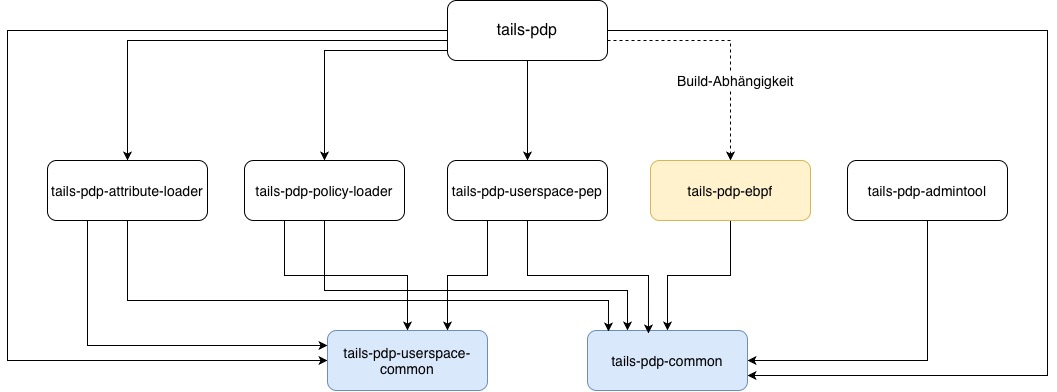
\includegraphics[width=0.95\textwidth]{graphics/abhaengigkeiten}
    \caption{Strukturelle Abhängigkeiten der projektinternen Rust-Crates}
    \label{fig:crate-abhaengigkeiten}
\end{figure}





\subsection{Gemeinsame Datenstrukturen und Map-ABI}
Die eBPF-Maps bilden die gemeinsame Datenschnittstelle zwischen Userspace und Kernelspace. Sie speichern Schlüssel und Werte als Bytefolgen, denen keine Rust-Typinformationen beigefügt sind. Damit ein im Userspace geschriebener Map-Eintrag vom eBPF-Programm eindeutig gelesen werden kann, müssen beide Ausführungsbereiche dieselbe Binärrepräsentation der verwendeten Datenstrukturen zugrunde legen. Dies betrifft insbesondere Feldreihenfolge, Feldgrößen und Ausrichtung der Schlüssel und Werte.

Diese gemeinsame Repräsentation bildet die Map-ABI des Prototyps. Die hierfür benötigten Strukturen sind in \path{tails-pdp-common} gebündelt und werden sowohl vom eBPF-Programm als auch von den Userspace-Komponenten verwendet. Die folgenden Unterabschnitte beschreiben die kernelgeeignete Darstellung von Policies und Attributen, die Identifikation von Ressourcen in Map-Schlüsseln sowie Aufbau und Pinning der verwendeten Maps. Das Einlesen, Validieren und Übersetzen der Policy- und Attributdateien wird dagegen in den nachfolgenden Abschnitten behandelt.

\subsubsection{Kernelgeeignete Policy-Strukturen}
Die Policy-Repräsentation ist auf eine konstante Größe und einen vorhersehbaren Kontrollfluss im eBPF-Programm ausgelegt. Für den Hook \texttt{file\_open} existieren deshalb getrennte Strukturen für statische und attributabhängige Policies. Beide Varianten enthalten die Zugriffsentscheidung, die Aktion, einen Aktivierungsstatus, das Subject sowie die Bedingungen für Kommando und Ressource. Kommando- und Ressourcenbezeichnungen werden dabei nicht als dynamische Zeichenketten, sondern als Arrays fester Länge abgelegt. Für Ressourcen werden zusätzlich Device- und Inode-Wert gespeichert.

Die Struktur \texttt{FileOpenStaticPolicy} enthält nur die Bedingungen, die unmittelbar mit dem Öffnungsvorgang verglichen werden können. \texttt{FileOpenStreamPolicy} erweitert diese Repräsentation um eine optionale Zeitbedingung und ein fest dimensioniertes Feld für Attributbedingungen. Jede dieser Bedingungen besteht aus Namespace, Vergleichsoperator, Werttyp, Hash des Attributnamens und dem Vergleichswert. Die Anzahl der aktiven Bedingungen wird gesondert gespeichert; das zugrunde liegende Array besitzt dennoch stets eine feste Obergrenze von vier Einträgen. Damit kann die Auswertung im eBPF-Programm mit begrenzten Schleifen erfolgen, ohne Speicher dynamisch reservieren zu müssen.

Beide Policy-Typen werden als Werte separater Array-Maps gespeichert. Nicht belegte Einträge werden mit einer deaktivierten Policy gefüllt. Die Trennung in statische und attributabhängige Policies erlaubt es, die Auswertung in getrennten Tail-Call-Stufen auszuführen. Die konkrete Aktivierung einer vollständigen Policy-Generation wird in Abschnitt~\ref{sec:policy-generation} beschrieben.

\subsubsection{Repräsentation dynamischer Attribute}
Das Attributmodell muss frei wählbare Namen und Werte abbilden, obwohl eBPF-Maps nur Strukturen fester Größe speichern können. Ein Attribut wird deshalb durch einen festen Schlüssel und einen typisierten Wert repräsentiert. \texttt{AttributeKey} enthält die aktive Attributbank, den Namespace, zwei Objektidentifikatoren und einen 128-Bit-Hash des Attributnamens. Der Schlüssel legt damit fest, zu welchem System-, Subject- oder Ressourcenobjekt ein Attribut gehört und unter welchem Namen es angesprochen wird.

\texttt{AttributeValue} unterscheidet numerische, boolesche und Zeichenkettenwerte. Zahlen und Wahrheitswerte werden direkt als \texttt{u64} gespeichert. Für Zeichenketten wird nicht der Text selbst, sondern sein 128-Bit-Hash abgelegt. Der Userspace validiert Attributnamen vor der Übernahme und akzeptiert ausschließlich ASCII-Buchstaben, Ziffern, Unterstriche und Bindestriche. Anschließend werden Name und gegebenenfalls Zeichenkettenwert mit derselben Hashfunktion in die feste Kernelrepräsentation übersetzt. Der Kernel muss daher weder Zeichenketten parsen noch dynamischen Speicher verwalten.

Die Policy-Struktur enthält zu jeder Attributbedingung denselben Namenshash sowie den erwarteten Wert. Bei der Auswertung erzeugt das eBPF-Programm aus der aktuellen Attributbank, dem Namespace und der Objektidentität einen \texttt{AttributeKey} und liest den zugehörigen Wert aus der Hash-Map. Fehlt ein erforderliches Attribut oder stimmt sein Typ beziehungsweise Vergleichswert nicht überein, gilt die Bedingung als nicht erfüllt. Details zum Einlesen und Validieren der \path{.attributes}-Dateien behandelt Abschnitt~\ref{sec:attribute-loading}.

\subsubsection{Objektidentitäten im Map-Schlüssel}
Die beiden Objektidentifikatoren im Attributschlüssel werden abhängig vom Namespace belegt. Für Systemattribute sind beide Werte null, da sie systemweit gelten. Subject-Attribute verwenden die numerische UID als primären Identifikator; der zweite Wert bleibt null. Ressourcenattribute verwenden dagegen Device- und Inode-Wert der Datei. Diese Zuordnung wird sowohl beim Einlesen der Attributdateien im Userspace als auch bei der eBPF-Auswertung verwendet.

Die Ressourcenidentität wird aus den Dateimetadaten ermittelt, nicht aus dem Pfadnamen. Der Pfad dient beim Attributloader lediglich dazu, die zugehörige Datei zu finden und ihre Metadaten auszulesen. In der Map werden Device und Inode als zwei getrennte \texttt{u64}-Werte gespeichert. Dadurch wird keine verkürzende Hash-Repräsentation der Ressourcenidentität verwendet und Dateien auf unterschiedlichen Dateisystemen bleiben unterscheidbar. Zugleich bleibt die Zuordnung bei Umbenennungen derselben Datei erhalten, solange Device und Inode unverändert bleiben.

Die Objektidentität ist Teil des Map-Schlüssels und damit Teil der ABI. Eine Änderung ihrer Größe, Reihenfolge oder Bedeutung würde den Aufbau der \path{ATTRIBUTES}-Map verändern. Bereits gepinnte Maps wären dann nicht mehr kompatibel und müssen vor dem Laden eines Programms mit dem geänderten Layout erkannt werden.

\subsubsection{Aufbau und Pinning der eBPF-Maps}
Tabelle~\ref{tab:pinned-map-abi} zeigt die gepinnten Maps, die den dauerhaften Datenaustausch zwischen den Komponenten ermöglichen. Die Policy- und Attributloader schreiben gültige Daten in diese Maps. Das eBPF-Programm liest sie bei der Zugriffsentscheidung; Userspace-PEP und Administrationstool öffnen dieselben Maps bei Bedarf erneut zur Überwachung beziehungsweise Anzeige.

\begin{table}[htbp]
    \centering
    \small
    \begin{tabular}{|p{4.2cm}|p{1.7cm}|p{3.4cm}|p{4.4cm}|}
        \hline
        \textbf{Map} & \textbf{Typ} & \textbf{Schlüssel und Wert} & \textbf{Aufgabe} \\
        \hline
        {\scriptsize\texttt{POLICY\_GENERATION}} & Array & \texttt{u32} $\rightarrow$ \texttt{u32} & Speichert die aktive Policy-Generation und bestimmt damit die auszuwertende Policy-Bank. \\
        \hline
        {\scriptsize\texttt{FILE\_OPEN\_STATIC\_POLICIES}} & Array & \texttt{u32} $\rightarrow$\newline {\scriptsize\texttt{FileOpenStaticPolicy}} & Enthält die statischen \texttt{file\_open}-Policies beider Policy-Banken. \\
        \hline
        {\scriptsize\texttt{FILE\_OPEN\_STREAM\_POLICIES}} & Array & \texttt{u32} $\rightarrow$\newline {\scriptsize\texttt{FileOpenStreamPolicy}} & Enthält die attribut- und zeitabhängigen \texttt{file\_open}-Policies beider Policy-Banken. \\
        \hline
        {\scriptsize\texttt{CURRENT\_TIME}} & Array & \texttt{u32} $\rightarrow$ \texttt{u64} & Stellt den aktuellen Unix-Zeitstempel für zeitabhängige Bedingungen bereit. \\
        \hline
        {\scriptsize\texttt{ATTRIBUTE\_GENERATION}} & Array & \texttt{u32} $\rightarrow$ \texttt{u32} & Speichert die aktive Attributgeneration und damit die aktive Attributbank. \\
        \hline
        {\scriptsize\texttt{ATTRIBUTES}} & Hash-Map & {\scriptsize\texttt{AttributeKey}} $\rightarrow$\newline {\scriptsize\texttt{AttributeValue}} & Enthält die dynamischen System-, Subject- und Ressourcenattribute. \\
        \hline
    \end{tabular}
    \caption{Gepinnte eBPF-Maps als Map-ABI des Prototyps}
    \label{tab:pinned-map-abi}
\end{table}

Beim Start legt \texttt{tails-pdp} das Pin-Verzeichnis \path{/sys/fs/bpf/tails-pdp} an und lädt das eBPF-Objekt mit diesem Verzeichnis als Standardpfad für Maps. Gepinnte Maps bleiben im BPF-Dateisystem erreichbar und können deshalb von später gestarteten Userspace-Komponenten über ihren Pfad geöffnet werden. Die nicht gepinnten Maps für Tail Calls, temporäre Entscheidungen und Debug-Konfiguration gehören dagegen ausschließlich zum geladenen eBPF-Objekt und sind nicht Teil der gemeinsamen Map-ABI.

Da gepinnte Maps einen Programmneustart überdauern können, prüft \texttt{tails-pdp} vor dem Laden des eBPF-Programms vorhandene Map-Layouts. Für jede ABI-relevante Map werden Schlüsselgröße, Wertgröße und maximale Eintragszahl mit den aktuellen Strukturdefinitionen verglichen. Bei einer Abweichung wird der Start abgebrochen, statt eine vorhandene Map mit einer möglicherweise falsch interpretierten Byte-Repräsentation weiterzuverwenden. Die Generationswechsel für Policies und Attribute bauen auf diesen stabilen Map-Layouts auf und werden in den jeweiligen Verarbeitungsabschnitten erläutert.

\subsection{Initialisierung und Laufzeitsteuerung}
\subsubsection{Laden und Prüfen des eBPF-Programms}
\subsubsection{Initialisierung der Maps und Tail Calls}
\subsubsection{Start der Userspace-Komponenten}

\subsection{Verarbeitung und Laden von Policies}
\subsubsection{Einlesen der Policydateien}
\subsubsection{Syntaktische Verarbeitung}
\subsubsection{Semantische Validierung}
\subsubsection{Übersetzung in Map-Einträge}
\subsubsection{Generationenwechsel und Rollback}\label{sec:policy-generation}

\subsection{Bereitstellung dynamischer Attribute}\label{sec:attribute-loading}
\subsubsection{Aufbau des Attributverzeichnisses}
\subsubsection{Parsen und Validieren der Attribute}
\subsubsection{Attributschlüssel und Hashwerte}
\subsubsection{Aktualisierung der Attributgeneration}
\subsubsection{Bereitstellung der Zeitinformation}

\subsection{Implementierung des Kernelspace-PEP}
\subsubsection{Verarbeitung des file\_open-Hooks}
\subsubsection{Tail-Call-Kette}
\subsubsection{Auswertung statischer Policies}
\subsubsection{Auswertung von Streampolicies}
\subsubsection{Combining und Durchsetzung}

\subsection{Implementierung des Userspace-PEP}
\subsubsection{Ermittlung bestehender Dateizugriffe}
\subsubsection{Erneute Policy-Auswertung}
\subsubsection{Entzug des betroffenen File Descriptors}

\subsection{Implementierung des Administrationstools}

\subsection{Fehlerbehandlung und Konsistenzsicherung}

\subsection{Build und Deployment auf dem Zielsystem}
\subsubsection{Cross-Compilation und Build-Artefakte}
\subsubsection{Implementierungsbedingte Grenzen}

\newpage

\section{Evaluation}\label{sec:evaluation}
Ziel der Evaluation ist es, zu untersuchen, ob der implementierte Prototyp die zentralen Prinzipien von ASBAC für Dateiöffnungen unter Linux wie vorgesehen umsetzt. Dazu werden die Verarbeitung von Policies und dynamischen Attributen, die Kontrolle neuer Dateiöffnungen sowie die Nachbewertung bereits bestehender Dateizugriffe überprüft. Zusätzlich werden der Laufzeitaufwand und die technischen Grenzen der prototypischen Umsetzung betrachtet.


\subsection{Testumgebung}

Die Evaluation erfolgt in einer ausschließlich für die Untersuchung verwendeten virtuellen
Maschine. Dadurch lassen sich die für das Laden der eBPF-Programme erforderlichen privilegierten
Operationen ausführen, ohne ein Produktivsystem zu beeinflussen. Während der privilegierten
End-to-End-Tests läuft keine weitere Instanz des Prototyps, da die Tests vorübergehend die
gepinnten BPF-Maps unter \mbox{\path{/sys/fs/bpf/tails-pdp}} verwenden. Die VM-Konfiguration, die
NixOS-Systemkonfiguration und die Definition der Entwicklungsumgebung werden gemeinsam mit dem
Quellcode archiviert. Die Dateien \path{nix-config/configuration.nix},
\path{nix-config/hardware-configuration.nix} und \path{nix-config/shell.nix} dokumentieren die
für die Evaluation relevanten System-, Hardwareerkennungs- und Werkzeugvoraussetzungen.

Für die Kernel- und Durchsetzungstests muss BPF in der aktiven LSM-Reihenfolge enthalten sein.
Darüber hinaus werden BTF-Informationen unter \mbox{\path{/sys/kernel/btf/vmlinux}} und ein unter
\mbox{\path{/sys/fs/bpf}}  eingehängtes BPF-Dateisystem vorausgesetzt. Das Laden und Anheften der
eBPF-Programme, der Zugriff auf die gepinnten Maps und der \texttt{ptrace}-basierte Entzug eines
File Descriptors benötigen erhöhte Berechtigungen. Root-Berechtigung und BTF-Verfügbarkeit werden
vom Testskript explizit geprüft; die Verfügbarkeit von BPF-LSM und BPF-Dateisystem wird durch den
erfolgreichen Runtime-Start, das Anhängen des Hooks und die erzeugten Map-Pins nachgewiesen.

\subsubsection{Hard- und Softwareumgebung}

Die virtuelle Maschine wird mittels QEMU/KVM auf einem Proxmox-VE-Host betrieben. Für die
Reproduzierbarkeit sind dabei zwei Perspektiven zu unterscheiden: Die von Proxmox ausgegebene
VM-Konfiguration beschreibt die vom Hypervisor bereitgestellten Ressourcen, während die von
NixOS erzeugte \path{hardware-configuration.nix} die im Gastsystem erkannten Geräte und die zu
ladenden Kernelmodule festhält. Keine der beiden Konfigurationen ersetzt daher vollständig die
jeweils andere.

Als virtuelles Prozessormodell ist \texttt{x86-64-v2-AES} konfiguriert. Zwei virtuelle Sockel mit
jeweils zwei Kernen stellen insgesamt vier virtuelle CPUs bereit; zusätzlich sind 8192~MiB
Arbeitsspeicher zugewiesen. Das virtuelle Systemlaufwerk besitzt eine Kapazität von 64~GiB und ist
über VirtIO-SCSI angebunden. Diese Angaben werden aus der VM-Konfiguration übernommen, weil sie
nicht Bestandteil der NixOS-Hardwarekonfiguration sind. Weitere betriebliche Kennungen und
Gerätedetails der VM sind für die durchgeführten Funktions- und Laufzeittests nicht
entscheidungsrelevant und werden daher nicht einzeln aufgeführt.

Als Gastbetriebssystem kommt NixOS zum Einsatz. Die archivierte Systemkonfiguration setzt
\texttt{system.stateVersion} auf \texttt{25.05}. Diese Option steuert kompatibilitätsrelevante
Voreinstellungen, um bestehende Anwendungsdaten bei Systemaktualisierungen weiterverwenden zu
können. Sie bezeichnet daher nicht die tatsächlich installierte NixOS-Version
\citep{nixosStateVersion}. Der Kernel wird durch die Konfiguration aus den Quellen des stabilen
Linux-Kernels 6.16.12 mit festgelegtem SHA-256-Hash gebaut. Auf dem Testsystem ist NixOS
\texttt{25.05.810656.5b5be50345d4} installiert. Die Konfiguration aktiviert unter
anderem die Kerneloptionen für das Security-Framework und SecurityFS. Die LSM-Auswahl wird
zentral über die NixOS-Option \texttt{security.lsm} auf \texttt{landlock}, \texttt{yama} und
\texttt{bpf} festgelegt. NixOS erzeugt daraus den Kernelparameter
\texttt{lsm=landlock,yama,bpf}. Zusammen mit dem vom Kernel ergänzten Capability-LSM ergibt
sich die auf dem Testsystem über \path{/sys/kernel/security/lsm} bestätigte aktive Reihenfolge
\texttt{capability,landlock,yama,bpf}.

Die von NixOS generierte \path{hardware-configuration.nix} bindet das QEMU-Gastprofil ein und
legt \texttt{x86\_64-linux} als Plattform des Gastsystems fest. Für den Systemstart werden unter
anderem die Module für VirtIO-PCI, VirtIO-SCSI und SCSI-Datenträger in die Initial Ramdisk
aufgenommen. Das Root-Dateisystem verwendet ext4, die EFI-Systempartition vfat.

Die Entwicklungs- und Build-Umgebung wird mit \texttt{nix-shell} aus
\path{nix-config/shell.nix} erzeugt. Für den regulären Projektbuild sind insbesondere Rustup und
Cargo, LLVM~21 einschließlich seiner Laufzeitbibliothek sowie \texttt{bpf-linker} erforderlich.
Der Shell-Hook wählt die Rust-Nightly-Toolchain \texttt{nightly-2025-08-01} einschließlich
\texttt{rust-src}, \texttt{rustfmt} und Clippy aus. Aya führt den Build der eBPF-Crate für das
Ziel \texttt{bpfel-unknown-none} aus. Das Build-Skript dieser Crate setzt die Verfügbarkeit des
\texttt{bpf-linker} voraus; die Shell-Konfiguration sieht dafür Version 0.9.15 mit
LLVM-21-Unterstützung vor. Die Rust-Abhängigkeiten werden durch \path{Cargo.lock} festgelegt; der
verwendete Stand enthält Aya 0.13.2 und \texttt{aya-ebpf} 0.1.2.

Für die Ausführung der Skripte enthält die Umgebung außerdem Bash, Coreutils, GNU Grep, Procps und
Python~3.

Tabelle~\ref{tab:testumgebung} fasst die aus den archivierten Konfigurationsdateien ableitbaren
Merkmale sowie die auf dem Testsystem ermittelte NixOS-Version und aktive LSM-Reihenfolge
zusammen. Die konkrete Proxmox-, NixOS-, Nixpkgs-, Rust- und Cargo-Version sowie der
getestete Git-Commit werden unmittelbar auf dem Testsystem erfasst und zusammen mit den
Testergebnissen dokumentiert. Dies ist insbesondere für Nixpkgs erforderlich, weil die aktuelle
\path{nix-config/shell.nix} das zum Ausführungszeitpunkt konfigurierte \texttt{<nixpkgs>}
importiert und keine feste Nixpkgs-Revision enthält.

\begin{table}[htbp]
    \centering
    \caption{Hard- und Softwarekonfiguration der Testumgebung}
    \label{tab:testumgebung}
    \begin{tabular}{p{0.36\textwidth}p{0.55\textwidth}}
        \hline
        \textbf{Komponente} & \textbf{Konfiguration} \\
        \hline
        Virtualisierungsplattform & Proxmox VE (9.2.18) mit QEMU/KVM \\
        Virtuelles CPU-Modell & \texttt{x86-64-v2-AES} \\
        CPU-Konfiguration & 4 vCPUs \\
        Arbeitsspeicher & 8192 MiB \\
        Virtuelles Laufwerk & 64 GiB \\
        Speicheranbindung & VirtIO-SCSI \\
        NixOS-Hardwareprofil & QEMU-Gast, Plattform \texttt{x86\_64-linux} \\
        Dateisysteme & ext4 für \path{/}, vfat für \path{/boot} \\
        Gastbetriebssystem & NixOS \texttt{25.05.810656.5b5be50345d4} \\
        Linux-Kernel & 6.16.12, aus festgelegtem Quellarchiv gebaut \\
        LSM-Reihenfolge & \texttt{capability,landlock,yama,bpf} \\
        Entwicklungsumgebung & \texttt{nix-shell} auf Basis von \texttt{<nixpkgs>} \\
        LLVM & LLVM-Paketfamilie 21 einschließlich \texttt{libLLVM} \\
        Rust-Toolchain & \texttt{nightly-2025-08-01} mit \texttt{rust-src} \\
        eBPF-Zielarchitektur & \texttt{bpfel-unknown-none} \\
        \texttt{bpf-linker} & 0.9.15 \\
        Aya / \texttt{aya-ebpf} & 0.13.2 / 0.1.2 gemäß \path{Cargo.lock} \\
        \hline
    \end{tabular}
\end{table}

Da die Evaluation innerhalb einer virtuellen Maschine erfolgt, können insbesondere Zeitmessungen
durch das Scheduling des Hypervisors und durch gleichzeitig auf dem Proxmox-Host ausgeführte
Arbeitslasten beeinflusst werden. Gemessene Laufzeiten charakterisieren daher die dokumentierte
Testumgebung und sind nicht ohne Weiteres als allgemeingültige Werte für andere Hard- und
Softwarekonfigurationen zu verstehen.

\subsection{Teststrategie und Testszenarien}

Die Evaluation kombiniert automatisierte Unit- und Komponententests mit privilegierten
End-to-End-Tests und ausgewählten Laufzeitmessungen. Die Teststufen liefern unterschiedliche
Arten von Evidenz und werden deshalb getrennt betrachtet. Unit- und Komponententests prüfen
isolierbare Logik unter kontrollierten Bedingungen. End-to-End-Szenarien untersuchen dagegen das
Zusammenspiel der Userspace-Komponenten mit den BPF-Maps und dem tatsächlich geladenen
eBPF-LSM-Programm. Die Laufzeitmessungen ergänzen die funktionalen Nachweise um quantitative
Aussagen zur Reaktionszeit und zum zusätzlichen Aufwand bei kontrollierten Dateiöffnungen.

Dieser Abschnitt beschreibt zunächst den Versuchsaufbau und das jeweils erwartete Verhalten. Die
tatsächlich beobachteten Resultate werden davon getrennt in Abschnitt~6.3 dargestellt. Dadurch
wird vermieden, die Bewertungskriterien nach Kenntnis der Ergebnisse anzupassen.

\subsubsection{Teststufen und Bewertungskriterien}

Die Unit-Tests untersuchen einzelne Funktionen mit fest vorgegebenen Eingaben und vergleichen deren
Ausgabe durch Assertions mit dem erwarteten Ergebnis. Komponententests beziehen mehrere Funktionen
einer Userspace-Komponente ein, ersetzen externe Abhängigkeiten jedoch teilweise durch
Testdoubles. So prüfen die Generationstests die Reihenfolge zwischen dem Schreiben in die inaktive
Bank und der anschließenden Aktivierung mit einem speicherbasierten Ersatz für die BPF-Maps.
Die Tests des Userspace-PEP verwenden einen
\texttt{FakeFdCloser}, der Schließversuche protokolliert, aber keinen realen Systemaufruf in einem
anderen Prozess ausführt. Diese Tests können die fachliche Logik und das lokale Fehlerverhalten
präzise prüfen, belegen jedoch weder die Annahme des eBPF-Programms durch den Kernel-Verifier noch
die reale Durchsetzung einer Zugriffsentscheidung.

Die End-to-End-Tests führen den vollständigen Pfad von einer Policy- oder Attributdatei über die
Loader und gepinnten BPF-Maps bis zur beobachtbaren Wirkung auf einen Dateizugriff aus. Sie prüfen
damit Eigenschaften, die sich in einer isolierten Testumgebung nicht nachweisen lassen, etwa das
Laden des eBPF-Objekts, das Anhängen des \texttt{file\_open}-Hooks und den tatsächlichen Entzug
eines File Descriptors. Quantitative Messungen werden wiederholt ausgeführt und anhand vorab
festgelegter Messgrößen ausgewertet. Einzelne erfolgreiche Durchläufe werden nicht als Nachweis
allgemeiner zeitlicher Garantien oder unbegrenzter Skalierbarkeit interpretiert.

Tabelle~\ref{tab:teststufen} fasst die Teststufen und ihre Aussagegrenzen zusammen.

\begin{table}[htbp]
    \centering
    \caption{Teststufen der Evaluation}
    \label{tab:teststufen}
    \begin{tabular}{p{0.22\textwidth}p{0.32\textwidth}p{0.37\textwidth}}
        \hline
        \textbf{Teststufe} & \textbf{Gegenstand} & \textbf{Aussagegrenze} \\
        \hline
        Unit-Test & Einzelne Parser-, Vergleichs- und Hilfsfunktionen & Kein realer Kernel- oder
        Durchsetzungsnachweis \\
        Komponententest & Zusammenwirkende Funktionen einer Userspace-Komponente, teilweise mit
        Testdoubles & Externe Schnittstellen wie BPF-Maps oder \texttt{ptrace} werden teilweise
        ersetzt \\
        End-to-End-Test & Vollständiger Pfad auf dem Linux-Zielsystem & Nachweis gilt für das
        definierte Szenario und die dokumentierte Testumgebung \\
        Laufzeitmessung & Reaktionszeit und Aufwand kontrollierter Dateiöffnungen & Keine
        allgemeine Echtzeit- oder Skalierbarkeitsgarantie \\
        \hline
    \end{tabular}
\end{table}

Für die abschließende Zuordnung zu den Anforderungen werden die Bewertungen \emph{erfüllt},
\emph{teilweise erfüllt} und \emph{nicht erfüllt} verwendet. Eine
Anforderung gilt als erfüllt, wenn ihr Akzeptanzkriterium unter den dokumentierten Bedingungen
vollständig beobachtet wird. Als teilweise erfüllt wird sie bewertet, wenn das vorgesehene
Grundverhalten nachweisbar ist, aber relevante Einschränkungen oder nicht abgedeckte Fälle
verbleiben. Schlägt das erwartete Verhalten fehl, gilt die Anforderung als nicht erfüllt.
Die Bewertung bezieht sich
stets auf den begrenzten Funktionsumfang des Prototyps und stellt keinen vollständigen
Sicherheitsnachweis dar.

\subsubsection{Unit- und Komponententests}

Das Skript \path{test.sh} bildet den zentralen Einstiegspunkt der gesamten Prüfkette. Sein erster,
nicht privilegierter Teil führt 61 automatisierte Rust-Tests in fünf Testbereichen aus. Die Option
\texttt{--locked} stellt sicher, dass Cargo dabei die
in \path{Cargo.lock} festgehaltene Abhängigkeitsauflösung nicht verändert. Der in der
Cargo-Konfiguration für reguläre Programmstarts eingestellte privilegierte Runner wird für diese
Tests durch \texttt{env} ersetzt. Die Tests benötigen daher keine Root-Rechte, laden kein
eBPF-Programm in den Kernel und verändern keine gepinnten BPF-Maps.

Die Tests der gemeinsamen Crate \path{tails-pdp-common} bilden mit 16 Testfällen die fachliche
Entscheidungslogik ab. Sie prüfen das Matching statischer und zeitabhängiger Policies, die
Ableitung von UTC-Komponenten, die Grenzen der Vergleichsoperatoren und die Combining-Regel
\emph{deny-overrides}. Darüber hinaus untersuchen sie dynamische Zahlen-, Boolean- und
Stringattribute, Typabweichungen sowie die unterschiedlichen Objektidentifikatoren der System-,
Subject- und Resource-Namespaces. Da Teile dieser Funktionen sowohl im Kernelspace- als auch im
Userspace-Pfad verwendet werden, prüfen die Tests die gemeinsam genutzte Semantik, nicht jedoch
die Einbindung in die jeweilige Laufzeitumgebung.

Der Policyloader besitzt 16 Tests für das Einlesen, Parsen, Übersetzen und Validieren textueller
Policies. Abgedeckt sind unter anderem statische und zeitabhängige Policies, frei benannte
dynamische Attribute, ungültige Attributnamen, doppelte Policynamen, fehlende Semikolons,
unbekannte oder deaktivierte Actions, ungültige Zeitwerte und das Überschreiten der festgelegten
Kapazitätsgrenzen. Zwei Tests prüfen für statische und dynamische Policies die Annahme von
Kommandonamen mit 15 Bytes und die Ablehnung von 16 Bytes, jeweils auch mit Zeichen, deren
UTF-8-Kodierung mehrere Bytes benötigt. Weitere Tests prüfen das rekursive Einlesen ausschließlich von Dateien mit der
Endung \path{.policy}. Ein speicherbasierter \texttt{FakePolicyStore} kontrolliert, dass zuerst
die inaktive Bank beschrieben und erst danach die neue Generation aktiviert wird. Simulierte
Schreib- und Aktivierungsfehler müssen die zuvor aktive Generation unverändert lassen; außerdem
werden nicht mehr belegte Einträge einer neu vorbereiteten Bank deaktiviert.

Die 13 Tests des Attributloaders prüfen das Parsen der unterstützten Zahlen-, Boolean- und
Stringwerte sowie die Validierung von Attributnamen und des zulässigen DEFCON-Wertebereichs.
Ergänzend werden ein vollständiges Verzeichnis mit System-, Subject- und Resource-Attributen sowie
die transaktionale Aktivierung einer neuen Attributbank mit simulierten Lösch-, Schreib- und
Aktivierungsfehlern untersucht. Weitere Fehlerfälle decken die Kapazitätsprüfung vor der ersten
Map-Änderung, Fehler beim Lesen von Generation und Belegung sowie die Fortsetzung des laufenden
Updaters nach einer fehlgeschlagenen Übernahme eines neuen Attributstands ab. Zwei
weitere Tests in \path{tails-pdp-userspace-common} untersuchen den begrenzten Trigger-Kanal. Sie
prüfen, dass mehrere schnell aufeinanderfolgende Aktivierungen bei voller Kanalkapazität
koalesziert werden und ein geschlossener Kanal als Fehler gemeldet wird.

Die 14 Tests des Userspace-PEP prüfen die Auswertung von Prozess- und
File-Descriptor-Informationen sowie die Steuerung der Nachbewertung. Dazu gehören das Filtern
numerischer Einträge unter \path{/proc}, die Auswahl der Real UID aus
\path{/proc/<pid>/status}, die Erkennung regulärer Dateien und die gezielte Zuordnung eines
Verstoßes zu Prozess und File Descriptor. Mit dem \texttt{FakeFdCloser} wird geprüft, dass ein
File Descriptor innerhalb eines Scans höchstens einmal behandelt wird, unterschiedliche
Deskriptoren unabhängig bleiben und ein fehlgeschlagener Schließversuch die Bearbeitung weiterer
Verstöße nicht abbricht. Ein zusätzlicher Test bildet die Konjunktion mehrerer dynamischer
Bedingungen im produktiven Lookup-Ablauf ab; ein weiterer weist nach, dass ein fehlgeschlagener
Entzug die Verarbeitung eines anderen Zielprozesses nicht verhindert. Ergänzend testen asynchrone
Fälle das Warten auf Aktivierungsereignisse sowie die Berechnung relevanter Stunden- und
Modulo-Zeitgrenzen.

Neben den funktionalen Rust-Tests führt der nicht privilegierte Teil von \path{test.sh} drei
Qualitätsprüfungen aus. Eine reine
Formatprüfung kontrolliert mit \texttt{cargo fmt}, ob der Rust-Quellcode dem vorgegebenen Format
entspricht. Clippy analysiert Produktions- und Testcode statisch; Warnungen werden dabei als
Fehler behandelt. Abschließend erzeugt ein Release-Build die Userspace-Binaries und über das
Build-Skript des Hauptprogramms auch das eingebettete eBPF-Objekt. Dieser Build belegt die
Übersetzbarkeit des gemeinsamen Quellstands, ersetzt aber nicht die anschließende Prüfung durch
den Kernel-Verifier. In der eBPF-Crate selbst werden keine nativen Unit-Tests ausgeführt, da ihr
Code für die BPF-Zielarchitektur und eine \texttt{no\_std}-Umgebung übersetzt wird. Die
gemeinsame Policylogik wird daher nativ getestet; die tatsächliche Kernelausführung ist
Gegenstand der folgenden End-to-End-Szenarien.

Ergänzend prüfen sechs nicht privilegierte Python-Tests die Laufzeit (PERF-03) Messauswertung. Sie prüfen
unter anderem die zeitliche Reihenfolge, fehlende oder mehrfache Zeitmarkierungen, eine
unvollständige Bündelungsphase und noch laufende Scans vor Messbeginn.

\subsubsection{Privilegierte End-to-End-Tests}

Die End-to-End-Prüfung wird auf dem in Abschnitt~6.1 beschriebenen Linux-Zielsystem mit
Root-Rechten ausgeführt. Der zentrale Runner \path{test.sh} fordert diese Berechtigungen nach dem
Release-Build über \texttt{sudo} an und ruft \path{tests/test-e2e.sh} auf. Dieses Skript bildet den
gemeinsamen Einstiegspunkt der End-to-End-Stufe und
ruft für die Test-IDs \texttt{E2E-01} bis \texttt{E2E-19} jeweils eine eigene Bashdatei unter
\path{tests/e2e/} auf. Vor dem Start bricht die Hauptdatei ab, wenn bereits eine Instanz des
Prototyps läuft; anschließend entfernt sie die bekannten Test-Maps unter
\path{/sys/fs/bpf/tails-pdp}. Deshalb darf die Suite ausschließlich auf dem dedizierten Testsystem
und nicht parallel zu einer regulären Instanz oder einem weiteren Testlauf ausgeführt werden.

Für die ersten zehn Szenarien startet die Hauptdatei eine gemeinsame Runtime in einem temporären
Arbeitsverzeichnis. Dieses enthält eigene Policy- und Attributverzeichnisse sowie eine geschützte
und eine nicht geschützte Testdatei. Änderungen werden zunächst vollständig in eine temporäre
Datei geschrieben und anschließend atomar aktiviert. Wo ein erlaubter Zugriff allein noch keinen
Nachweis für die Verarbeitung einer Änderung liefern würde, wartet der Test zusätzlich auf einen
Wechsel der Policy- oder Attributgeneration. Nach \texttt{E2E-10} wird diese Runtime beendet und
der gepinnte Testzustand entfernt.

Die Szenarien \texttt{E2E-11} bis \texttt{E2E-19} werden darin anschließend über
\path{tests/test-evaluation.sh} mit jeweils eigener Runtime und isoliertem Arbeitsverzeichnis
ausgeführt. Der zugehörige Runner sperrt parallele Evaluationsläufe, verwaltet ausschließlich die
von ihm gestarteten Prozesse und verweigert den Start, wenn bekannte gepinnte Maps bereits
vorhanden sind. Beim Aufräumen entfernt er nur die durch den jeweiligen Lauf erzeugten Maps. Für
die Prüfung neuer Dateiöffnungen verwendet dieser Teil der Suite einen kleinen Syscall-Helfer. Ein
Zugriff gilt nur dann als durch den LSM-Hook verweigert, wenn \texttt{open()} mit \texttt{EPERM}
fehlschlägt; andere Ein-/Ausgabefehler werden nicht als erfolgreiches Deny gewertet.

Die Kennungen der ergänzenden Szenarien unterscheiden Komponententests (COMP),
Charakterisierungstests (CHAR), Tests auf Wettlaufsituationen (RACE), Laufzeitmessungen (PERF),
Kapazitätstests (LOAD) und Stabilitätstests (STAB). Die nachgestellte Nummer identifiziert das
jeweilige Szenario innerhalb der Testgruppe.

Nach Abschluss aller 19 End-to-End-Szenarien ruft \path{test.sh} denselben Evaluationsrunner ein
zweites Mal ausschließlich für \texttt{COMP-04}, \texttt{CHAR-01}, \texttt{RACE-01},
\texttt{PERF-01} bis \texttt{PERF-03}, \texttt{LOAD-01} und \texttt{STAB-01} auf. Damit werden
alle Teststufen durch einen Aufruf von \path{test.sh} ausgeführt, ohne die Szenarien
\texttt{E2E-11} bis \texttt{E2E-19} doppelt zu starten. Die Teilrunner bleiben für gezielte
Wiederholungen einzelner Szenarien separat aufrufbar.

Tabelle~\ref{tab:e2e-basis} fasst die grundlegenden Start-, Entscheidungs- und Attributszenarien
zusammen. Die Kriterien beschreiben den vorab erwarteten Zustand; die tatsächlich beobachteten
Ergebnisse werden getrennt in Abschnitt~6.3 berichtet.

\begin{table}[htbp]
    \centering
    \caption{Grundlegende End-to-End-Szenarien}
    \label{tab:e2e-basis}
    \begin{tabular}{p{0.16\textwidth}p{0.34\textwidth}p{0.41\textwidth}}
        \hline
        \textbf{Test-ID} & \textbf{Gegenstand} & \textbf{Bestehenskriterium} \\
        \hline
        E2E-01 & Runtime, Kernel-Verifier, LSM-Attach und Maps & Die Runtime bleibt aktiv und alle
        erwarteten Maps sind gepinnt. \\
        E2E-02 bis E2E-04 & Standardentscheidung, statische Deny-Policy und aktuelle UTC-Stunde &
        Der Zugriff ist ohne passende Deny-Policy erlaubt, wird bei passender statischer oder
        zeitabhängiger Policy verweigert und nach deren Entfernung wieder erlaubt. \\
        E2E-05 bis E2E-07 & System-, Subject- und Resource-Attribute & Änderungen von
        \texttt{system.defcon}, \texttt{subject.position} und
        \texttt{resource.classification} verändern die reale Zugriffsentscheidung in beide
        Richtungen. \\
        E2E-08 & Ungültige Policygeneration & Die Runtime meldet den Parserfehler, aktiviert die
        fehlerhafte Generation nicht und erzwingt weiterhin die letzte gültige Deny-Policy. \\
        E2E-12 & Konjunktion mehrerer Attribut-Namespaces & Die Deny-Policy greift nur bei
        gleichzeitig passenden System-, Subject- und Resource-Attributen; fehlende, typfalsche
        oder abweichende Einzelwerte heben das Deny auf. \\
        E2E-13 & Ungültige Attributgeneration & Ein unzulässiger Attributwert wird gemeldet, ohne
        die sichtbare Generation oder die zuvor gültige Entscheidung zu verändern. \\
        \hline
    \end{tabular}
\end{table}

Die weiteren Szenarien in Tabelle~\ref{tab:e2e-enforcement} konzentrieren sich auf die
Combining-Regel, bestehende File Descriptors, die Administrationsschnittstelle und kontrollierte
Fehlerfälle. Beim nachträglichen Entzug hält ein Hilfsprozess mehrere Deskriptoren geöffnet und
prüft über \texttt{fstat()}, ob ausschließlich die von der neuen Entscheidung betroffenen
Deskriptoren ungültig werden. Der Fehlercode \texttt{EBADF} (\emph{Bad file descriptor},
ungültiger Dateideskriptor) zeigt dabei an, dass der geprüfte Deskriptor nicht mehr gültig ist
\citep{manErrno}.

\begin{table}[htbp]
    \centering
    \caption{End-to-End-Szenarien für Enforcement und Fehlerverhalten}
    \label{tab:e2e-enforcement}
    \begin{tabular}{p{0.16\textwidth}p{0.34\textwidth}p{0.41\textwidth}}
        \hline
        \textbf{Test-ID} & \textbf{Gegenstand} & \textbf{Bestehenskriterium} \\
        \hline
        E2E-09 und E2E-16 & Selektiver Entzug bestehender File Descriptors & Ein beziehungsweise
        mehrere verletzende Deskriptoren werden geschlossen; weiterhin zulässige Deskriptoren
        desselben Prozesses bleiben geöffnet. \\
        E2E-10 und E2E-14 & Administrationsschnittstelle und Nachvollziehbarkeit & Die Ausgabe
        enthält aktive Generation, Deny-Policy, Ressourcenidentität, Attributbedingung und
        Attributwert, ohne den Zustand zu verändern. Dies weist die rekonstruierbare Ursache im
        kontrollierten Szenario nach, jedoch kein individuelles Auditlog jeder Entscheidung. \\
        E2E-11 & Combining-Regel \emph{deny-overrides} & Bei gleichzeitig passender Permit- und
        Deny-Policy wird der Zugriff unabhängig von der lexikalischen Policyreihenfolge verweigert;
        nach Entfernen des Deny wird er erlaubt. \\
        E2E-15 & Real und Effective UID & Bei privilegiertem Effective- und Filesystem-User wird
        die Entscheidung anhand der gesetzten Real UID getroffen; eine andere Real UID bildet die
        Negativkontrolle. \\
        E2E-17 & Nicht erreichbarer Zielprozess beim FD-Entzug & Der gezielt erzeugte
        \texttt{ptrace}-Attach-Konflikt wird protokolliert, ein anderer Zielprozess wird dennoch
        verarbeitet und weitere Policyaktivierungen sowie Kernelentscheidungen bleiben möglich. \\
        E2E-18 & Attributgetriggerter FD-Entzug & Eine reine Attributänderung schließt drei
        unzulässige FDs; zwei erlaubte bleiben offen. Die Policygeneration bleibt unverändert. \\
        E2E-19 & Zeitgetriggerter FD-Entzug & Eine Zeitgrenze schließt drei unzulässige FDs;
        zwei erlaubte bleiben offen. Policy- und Attributgeneration bleiben unverändert. \\
        \hline
    \end{tabular}
\end{table}

Ein Szenario gilt nur dann als bestanden, wenn sein Skript ohne fehlgeschlagene Assertion endet,
die Runtime während der vorgesehenen Prüfung aktiv bleibt und im neu hinzugekommenen Kernel-Log
kein Hinweis auf \emph{Kernel panic}, \emph{Oops}, \emph{BUG} oder einen General-Protection-Fault
enthalten ist. Für die isolierten Szenarien werden Status, Parameter und gegebenenfalls erzeugte
Detaildaten in \path{report.json} gespeichert. Runtime-, Szenario- und Kernel-Logs bleiben im
ausgegebenen Verzeichnis unter \path{/tmp/tails-eval-*} erhalten. Diese Artefakte bilden die
Grundlage für die Ergebnisdarstellung, sind aber selbst noch kein Nachweis über andere Kernel,
Konfigurationen oder Lastsituationen hinaus.
Die Nachweise der hier ausgewerteten Prüfkette sind einschließlich Gesamtprotokoll,
Szenarioberichten, Messrohwerten und Umgebungsangaben unter
\path{thesis/test-results/final-evaluation/} archiviert.

\clearpage
\subsection{Ergebnisse}

Die nachfolgend dargestellten Ergebnisse wurden auf dem in Abschnitt~6.1 beschriebenen
Zielsystem erhoben.

\subsubsection{Ergebnisse der funktionalen Prüfungen}

Alle 61 Unit- und Komponententests wurden erfolgreich ausgeführt. Davon entfallen 16 Tests auf
die gemeinsame Policylogik, 16 auf den Policyloader, 13 auf den Attributloader, zwei auf den
gemeinsamen Triggerkanal und 14 auf den Userspace-PEP. Die Formatprüfung und der separate
Release-Build der Runtime und des Administrationstools einschließlich des eBPF-Objekts waren
ebenfalls erfolgreich. Damit ist nachgewiesen, dass der Prototyp übersetzbar ist
und die in Abschnitt~6.2.2 beschriebenen Assertions erfüllt.

Die vollständige Ausführung von \path{test.sh} wurde mit Exitstatus null abgeschlossen.
Clippy prüfte Produktions-, Test- und Binärziele mit als Fehler behandelten Warnungen erfolgreich.
Auch die sechs ergänzenden Python-Tests zur Auswertung der PERF-03-Zeitmarkierungen bestanden.
Alle acht ergänzenden Evaluationsszenarien für Map-Zugriff, Deskriptorgrenzen, Race-Verhalten,
Performance, Kapazität und Stabilität wurden ebenfalls erfolgreich abgeschlossen.
Damit waren sowohl die funktionalen Prüfungen als auch die definierte Qualitätsprüfkette
vollständig erfolgreich.

Auf dem Zielkernel bestanden alle 19 End-to-End-Szenarien. Die Runtime wurde vom
Kernel-Verifier akzeptiert, der \texttt{file\_open}-Hook angehängt und die erwarteten Maps wurden
gepinnt. Ohne passende Deny-Policy blieb der Zugriff erlaubt; statische, zeitabhängige und von
dynamischen Attributen abhängige Deny-Policies führten dagegen zu \texttt{EPERM}. Änderungen von
System-, Subject- und Resource-Attributen wurden in beide Entscheidungsrichtungen übernommen.
Auch die Konjunktion mehrerer Attribut-Namespaces und die Combining-Regel
\emph{deny-overrides} zeigten das erwartete Verhalten.

Ungültige Policy- und Attributstände ersetzten die jeweils letzte gültige Generation nicht.
Nach der Korrektur des Attributloaders wurde auch eine Überschreitung der realen Map-Kapazität
kontrolliert abgelehnt: Je 512 Attribute pro vollständig belegter Bank wurden akzeptiert, ein
Update auf 513 Attribute bei weiterhin 512 Einträgen der aktiven Bank dagegen vor einer
Veränderung der Maps zurückgewiesen. Generation und aktive Attributwerte blieben unverändert;
anschließende gültige Updates wurden ohne Neustart der Runtime verarbeitet. Für Policies wurden
je 16 statische und 16 Stream-Policies akzeptiert und der jeweils 17. Eintrag kontrolliert
abgelehnt. Damit wurde nicht nur das Verhalten an den vorgesehenen Grenzen, sondern auch die
Wiederherstellung des regulären Updatebetriebs nach einer Ablehnung beobachtet.

Der nachträgliche Entzug bestehender Dateizugriffe war in den vorgesehenen Szenarien ebenfalls
erfolgreich. Sowohl ein einzelner als auch drei gleichzeitig verletzende File Descriptors wurden
geschlossen, während die erlaubten Deskriptoren desselben Prozesses geöffnet blieben.
E2E-18 bestätigte dieses Verhalten nach einer reinen Attributänderung bei unveränderter
Policygeneration. E2E-19 bestätigte es beim Erreichen einer Zeitgrenze ohne Änderung der
Policy- und Attributgeneration. In beiden Szenarien wurden drei unzulässige Deskriptoren
geschlossen, während zwei erlaubte geöffnet blieben. War ein
Zielprozess aufgrund eines bestehenden \texttt{ptrace}-Attachs nicht erreichbar, wurde der
Fehler protokolliert und ein weiterer Prozess trotzdem erfolgreich verarbeitet. Nachfolgende
Policyaktivierungen und Kernelentscheidungen blieben möglich. Die Administrationsschnittstelle
zeigte aktive Generationen, Policies, Ressourcen und Attribute ohne beobachtete Zustandsänderung.
Im kontrollierten Szenario ließ sich die Ursache einer Ablehnung aus der einzigen aktiven
Deny-Policy, der Ressourcenidentität, der Attributbedingung und dem aktuellen Attributwert
rekonstruieren. Ein individuelles Entscheidungsprotokoll für jede Dateiöffnung oder der
ursprüngliche Policyname wird jedoch nicht ausgegeben.

\begin{table}[htbp]
    \centering
    \caption{Zusammenfassung der funktionalen Testergebnisse}
    \label{tab:funktionale-ergebnisse}
    \begin{tabular}{p{0.28\textwidth}p{0.18\textwidth}p{0.45\textwidth}}
        \hline
        \textbf{Prüfung} & \textbf{Ergebnis} & \textbf{Einordnung} \\
        \hline
        Rust-Tests & 61 von 61 bestanden & Unit- und Komponentennachweise ohne realen
        Kernelpfad \\
        End-to-End-Tests & 19 von 19 bestanden & Vollständiger Pfad einschließlich
        Kernel-Verifier, LSM-Attach und Enforcement \\
        Formatprüfung & Bestanden & Keine Formatabweichungen im Rust-Code \\
        Python-Tests & 6 von 6 bestanden & Prüfung der PERF-03-Messauswertung \\
        Clippy-Gesamtprüfung & Bestanden & Statische Analyse mit als Fehler behandelten
        Warnungen \\
        Release-Build & Bestanden & Userspace-Binaries und eBPF-Objekt wurden erzeugt \\
        Kapazitätstest & Bestanden & Kontrollierte Ablehnung ohne Zustandsverlust und mit
        erfolgreichen Folgeupdates \\
        \hline
    \end{tabular}
\end{table}

\subsubsection{Robustheit und Grenzen des Entzugsmechanismus}

Im Stabilitätstest wurden 100 aufeinanderfolgende Zyklen mit gültigen und ungültigen Policy- und
Attributänderungen ausgeführt. Die Runtime blieb bis zum regulären Testende aktiv. Die vom Runner
ausgewertete Differenz des Kernel-Logs enthielt keinen Hinweis auf Kernel-Panic, Oops, BUG oder
einen General-Protection-Fault. Der Abschlusslauf benötigte 175~Sekunden. Dieses Ergebnis
belegt das Verhalten während des begrenzten Tests, stellt jedoch weder einen Langzeittest noch
einen allgemeinen Nachweis der Kernelstabilität dar.

Die Charakterisierung duplizierter und durch \texttt{fork()} vererbter Deskriptoren zeigte, dass
in Eltern- und Kindprozess jeweils alle vier betroffenen Deskriptoren geschlossen wurden, während
jeweils zwei erlaubte Deskriptoren geöffnet blieben. Eine bereits bestehende
\texttt{mmap()}-Abbildung der Datei blieb danach lesbar. Der Prototyp entzieht somit den File
Descriptor, widerruft aber keinen zuvor eingerichteten speicherabgebildeten Zugriff. Diese Grenze
folgt aus dem in Kapitel~3 ausdrücklich auf File Descriptors eingegrenzten Prototypumfang, ist
für die sicherheitstechnische Interpretation des Ergebnisses jedoch relevant.

Im nebenläufigen Stresstest wurden während zehn Policyzyklen 5387 Wechsel der Ressource hinter
derselben Deskriptornummer erzeugt. Dabei wurde kein erlaubter Deskriptor fälschlich geschlossen.
Da der Test stochastisch ist, beweist dieses Ergebnis keine Race-Freiheit. Zwischen dem Erfassen
der Deskriptoridentität und dem späteren \texttt{ptrace}-basierten Schließen verbleibt grundsätzlich
ein Zeitfenster, in dem der Zielprozess die Deskriptornummer wiederverwenden kann.

\subsubsection{Quantitative Ergebnisse}

Tabelle~\ref{tab:performance-ergebnisse} enthält die zentralen Messwerte. Bei PERF-01 wurden je
20\,000 Dateiöffnungen mit warmem Cache gemessen. Jeder der drei Messzustände wurde zuvor
mit 1000 ungemessenen Öffnungs- und Schließvorgängen vorbereitet. Der Median stieg von
3,512~$\mu$s ohne aktiven Prototyp auf 3,985~$\mu$s mit aktivem Prototyp ohne Policy und auf
4,014~$\mu$s bei passender Permit-Policy. Dies entspricht einem medianen Mehraufwand von
13,5 beziehungsweise 14,3~Prozent. Die Messung umfasst \texttt{os.open()} sowie den Aufwand der
Python-Laufzeit und des Timers; \texttt{close()} liegt außerhalb des Messintervalls. Sie isoliert
daher nicht ausschließlich die Ausführungszeit des LSM-Hooks.

\begin{table}[htbp]
    \centering
    \caption{Quantitative Messergebnisse auf dem Zielsystem}
    \label{tab:performance-ergebnisse}
    \begin{tabular}{p{0.40\textwidth}p{0.13\textwidth}p{0.17\textwidth}p{0.17\textwidth}}
        \hline
        \textbf{Messgröße} & \textbf{$n$} & \textbf{Median} & \textbf{p95} \\
        \hline
        Dateiöffnung ohne Runtime & 20\,000 & 3,512~$\mu$s & 3,670~$\mu$s \\
        Dateiöffnung, Runtime ohne Policy & 20\,000 & 3,985~$\mu$s & 4,104~$\mu$s \\
        Dateiöffnung, passende Permit-Policy & 20\,000 & 4,014~$\mu$s & 4,195~$\mu$s \\
        Policyänderung bis neues Deny & 10 & 104,42~ms & 114,75~ms \\
        Attributänderung bis neues Deny & 10 & 99,17~ms & 104,57~ms \\
        Policyänderung bis \texttt{EBADF} & 10 & 110,43~ms & 112,24~ms \\
        \hline
    \end{tabular}
\end{table}

Die Reaktionszeit vom atomaren Austausch einer Datei bis zur beobachtbaren neuen Entscheidung
lag im Median bei 104,42~ms für Policyänderungen und 99,17~ms für Attributänderungen. Dabei wurde
der Zugriff in Intervallen von 10~ms geprüft. Die Messung enthält somit neben Verarbeitung und
Aktivierung auch Dateisystembeobachtung, Scheduling und Polling.

Für den Entzug bestehender Zugriffe betrug die Zeit von der Policydateiänderung bis zum
beobachteten \texttt{EBADF} im Median 110,43~ms. PERF-03 bereitet die Policydatei außerhalb
des überwachten Verzeichnisses vor und beginnt die Messung unmittelbar vor ihrer atomaren
Umbenennung in das Policyverzeichnis. Zuvor müssen der wartende Policy-Watcher und abgeschlossene
Scans über 300~ms einen unveränderten Ruhezustand zeigen. Zeitmarkierungen prüfen, dass das
Dateiereignis erst nach Messbeginn empfangen und die vollständige 100-ms-Bündelungsphase
abgewartet wurde. Zwei weitere Zeitmarkierungen unmittelbar vor und nach dem Map-Systemaufruf
zur Aktivierung grenzen deren Zeitpunkt ein. Die Messung enthält den Aufwand dieser
Instrumentierung; der Entzug wird durch FD-Prüfungen im Abstand von 1~ms beobachtet.
Über zehn Wiederholungen lagen die unteren Grenzen der Aktivierung-bis-Entzug-Intervalle
zwischen 8,09 und 10,22~ms, die oberen Grenzen zwischen 8,10 und 10,25~ms. Eine scheinexakte
Einzelzeit wird daraus nicht abgeleitet. Bei nur zehn Wiederholungen entspricht das angegebene p95 jeweils dem beobachteten
Maximum und ist keine belastbare Schätzung seltener Ausreißer. Da für OA-03 keine feste
Latenzgrenze vorgegeben wurde, bedeutet ein bestandener Performance-Test ausschließlich, dass die
Messung erfolgreich durchgeführt und der Zustandswechsel beobachtet wurde.

\subsubsection{Bewertung der Anforderungen}

Die funktionalen Anforderungen FA-01 bis FA-10 werden innerhalb des in Kapitel~3 definierten
Prototypumfangs als erfüllt bewertet. Die Tests weisen das Einlesen, Aktualisieren und Validieren
von Policies, die Kontrolle neuer Dateiöffnungen, dynamische und frei benannte Attribute sowie
den selektiven Entzug unzulässig gewordener File Descriptors nach. Diese Bewertung umfasst nur
die getesteten Policyformen, Attributtypen und den Hook \texttt{file\_open}.
Bei FA-06 bezieht sich die Erfüllung auf die geforderte Nachbewertung und den gezielten
Schließversuch einschließlich kontrollierter Fehlerbehandlung. E2E-09 und E2E-16 zeigen den
erfolgreichen selektiven Entzug nach einer Policyänderung. E2E-18 und E2E-19 weisen ihn außerdem
nach einer reinen Attributänderung beziehungsweise beim Erreichen einer Zeitgrenze nach.
E2E-17 zeigt, dass ein fehlgeschlagener
Versuch bei einem nicht erreichbaren Zielprozess protokolliert wird und die Behandlung eines
anderen Zielprozesses nicht verhindert. Der im Fehlerfall verbleibende offene Deskriptor ist
damit eine Grenze des Best-Effort-Entzugs, bei dem das Schließen versucht, aber nicht garantiert
wird. Ein im Fehlerfall offen gebliebener Deskriptor gilt nicht als erfolgreich entzogen. Die Bewertung besagt nicht,
dass jeder unzulässig gewordene Zugriff erfolgreich beendet werden kann. Insbesondere folgt
aus FA-06 kein Widerruf bestehender \texttt{mmap()}-Abbildungen, da der bestehende Zugriff dort für
den Prototyp explizit als geöffneter File Descriptor definiert ist. Die beobachtete
Entzugslatenz ist außerdem keine Echtzeitgarantie.

OA-01 wird für die untersuchten Eingaben und die Dauer der Testläufe erfüllt. Ungültige Eingaben,
Kapazitätsüberschreitungen und ein nicht erreichbarer Zielprozess führten in den Abschlussläufen
weder zum Abbruch der Runtime noch zu einem vom Runner erkannten Kernelproblem. Eine allgemeine
Stabilitätsgarantie kann daraus nicht abgeleitet werden. OA-02 ist teilweise erfüllt: Die
Administrationsschnittstelle ermöglicht im kontrollierten Szenario eine Rekonstruktion der
Entscheidungsgrundlage, stellt aber kein individuelles Auditlog bereit und ordnet eine konkrete
Dateiöffnung nicht unmittelbar einem ursprünglichen Policynamen zu. OA-03 ist erfüllt, weil der
zusätzliche Aufwand und die Reaktions- und Entzugslatenz quantitativ untersucht wurden.
OA-04 wird durch die archivierten Konfigurationen,
Szenarioskripte, Testparameter und Rohdaten erfüllt.

Die entwicklungsbezogenen Anforderungen sind nicht allein durch Laufzeittests entscheidbar. Die
Trennung in eBPF-Programm, gemeinsame Datentypen und Entscheidungslogik, Loader,
Userspace-PEP und Administrationstool unterstützt EA-01. Frei benannte Attribute und getrennte
Komponenten bieten Erweiterungspunkte im Sinne von EA-02; neue Attributtypen, Map-Strukturen oder
LSM-Hooks erfordern jedoch weiterhin Änderungen an mehreren Schnittstellen, weshalb diese
Anforderung nur teilweise erfüllt ist. EA-03 wird dadurch unterstützt, dass Einlesen,
Validierung, Aktualisierung, Nachbewertung und Administration im Userspace liegen. Im Kernel
verbleiben der notwendige LSM-Hook, Map-Lookups und die unmittelbar für eine Dateiöffnung
erforderliche Auswertung.

Insgesamt zeigen die Ergebnisse, dass der Prototyp die für diese Arbeit ausgewählten
ASBAC-Prinzipien auf dem untersuchten Linux-System funktional umsetzt: Zugriffsentscheidungen
reagieren auf Policy- und Attributströme, neue Dateiöffnungen werden im Kernel kontrolliert und
bereits geöffnete File Descriptors im Userspace nachbewertet. Die Ergebnisse sind ein
Machbarkeitsnachweis für den definierten Prototyp, kein vollständiger Sicherheits-,
Race-Freiheits-, Echtzeit- oder Produktionstauglichkeitsnachweis.

\newpage

\section{Zusammenfassung und Ausblick}

\subsection{Zusammenfassung und Beantwortung der Forschungsfrage}

Diese Arbeit untersuchte, wie zentrale Prinzipien von Attribute Stream-Based Access Control für Dateiöffnungen prototypisch mittels eBPF-LSM unter Linux umgesetzt werden können und welche technischen Einschränkungen sich insbesondere bei der nachträglichen Kontrolle bestehender Dateizugriffe ergeben. Hierzu wurde ein Prototyp entwickelt, der textuelle Policies und dynamische Attribute im Userspace verarbeitet, in eine feste Kernelrepräsentation übersetzt und über gepinnte eBPF-Maps bereitstellt. Neue Dateiöffnungen werden unmittelbar im LSM-Hook \texttt{file\_open} bewertet. Bereits geöffnete File Descriptors werden nach einer erfolgreichen Policy- oder Attributaktivierung sowie beim Erreichen einer entscheidungsrelevanten Zeitgrenze im Userspace erneut untersucht. Ergibt die Nachbewertung eine Verletzung, versucht der Userspace-PEP, den betroffenen Deskriptor im Zielprozess zu schließen.

Die Forschungsfrage lässt sich damit wie folgt beantworten: Eine prototypische Übertragung ausgewählter ASBAC-Prinzipien ist durch eine hybride Architektur möglich. eBPF-LSM bildet einen kernelgestützten Durchsetzungspfad für neue Dateiöffnungen, während Userspace-Komponenten die komplexere Policyverarbeitung, die Aktualisierung dynamischer Attribute und die Nachkontrolle bestehender Deskriptoren übernehmen. Feste Datentypen und begrenzte Kontrollflüsse machen die Entscheidungslogik für eBPF ausführbar. Zwei Map-Bänke und getrennte Generationszähler sorgen dafür, dass neue Policy- und Attributstände erst nach ihrer vollständigen Vorbereitung aktiviert werden. Die Aufteilung über Tail Calls begrenzt die Komplexität der einzelnen eBPF-Programme. Kernelspace-PEP und Userspace-PEP verwenden dieselbe Policysemantik, dieselben Objektidentitäten und die Real UID als definierte Subjektidentität.

Die Evaluation bestätigt die technische Machbarkeit für den untersuchten Funktionsumfang und das dokumentierte Zielsystem. Alle 59 Unit- und Komponententests sowie alle 17 privilegierten End-to-End-Szenarien bestanden. Dabei wurden unter anderem statische und dynamische Deny-Entscheidungen, die Combining-Regel \emph{deny-overrides}, konsistente Generationenwechsel, die kontrollierte Ablehnung ungültiger Zustände und der selektive Entzug bestehender File Descriptors beobachtet. Der Kernel-Verifier akzeptierte das eBPF-Programm, und der LSM-Hook wurde erfolgreich angehängt. Die UID-Semantik stimmte auch bei voneinander abweichenden Real- und Effective-UIDs mit der festgelegten Real-UID-Semantik überein.

Die Laufzeitmessungen zeigen zugleich, dass die zusätzliche Kontrolle nicht kostenfrei ist. Der Median einer gemessenen Dateiöffnung stieg in der verwendeten Testumgebung von 3,845~$\mu$s ohne Runtime auf 4,389~$\mu$s bei aktiver Runtime ohne Policy und auf 4,412~$\mu$s bei einer passenden Permit-Policy. Dies entspricht in diesem Versuchsaufbau einem medianen Mehraufwand von 14,1 beziehungsweise 14,7~Prozent. Policy- und Attributänderungen beeinflussten neue Entscheidungen im Median nach rund 102 beziehungsweise 103~ms. Vom Austausch einer Policydatei bis zum beobachteten \texttt{EBADF} eines zuvor geöffneten Deskriptors vergingen im Median 58,91~ms. Diese Werte charakterisieren die dokumentierte virtuelle Testumgebung; sie stellen weder eine Echtzeitgarantie noch einen isolierten Mikrobenchmark ausschließlich des LSM-Hooks dar.

Insgesamt erreicht der Prototyp damit das Ziel eines Machbarkeitsnachweises. Er zeigt, wie dynamische Entscheidungsgrundlagen in einen eBPF-LSM-Pfad einbezogen und bestehende Deskriptoren nach relevanten Zustandsänderungen erneut bewertet werden können. Er implementiert jedoch weder die vollständige Publish-Subscribe-Architektur von SAPL noch einen allgemeinen eigenständigen ASBAC-PDP. Ein geöffneter File Descriptor wird nicht als Subscription verwaltet, sondern bei einem Auslöser erneut aus dem zu diesem Zeitpunkt sichtbaren Systemzustand rekonstruiert. Die Bezeichnungen Kernelspace-PEP und Userspace-PEP beschreiben die jeweilige Durchsetzungsfunktion; beide Komponenten enthalten zugleich die für ihren Pfad erforderlichen Funktionen zur Policyentscheidung.

\subsection{Grenzen der Ergebnisse}

Die stärkste Durchsetzung bietet der Kernelspace-PEP für den eng definierten Zeitpunkt einer neuen Dateiöffnung. Die nachträgliche Behandlung eines bestehenden Zugriffs ist dagegen eine ereignisbasierte Best-Effort-Maßnahme. Das Durchlaufen von \path{/proc}, die erneute Policybewertung und der mittels \texttt{ptrace} ausgeführte \texttt{close}-Systemaufruf bilden keine atomare Operation. Zwischen Identifikation und Entzug kann der Zielprozess eine Deskriptornummer schließen oder neu belegen. Der nebenläufige Stresstest beobachtete zwar keinen Fehlentzug, kann Race-Freiheit aber nicht beweisen. Ein nicht erreichbarer Zielprozess kann nicht zum Schließen seines Deskriptors gezwungen werden.

Das Schließen eines File Descriptors beendet außerdem nicht jede Nutzung, die aus einer früheren Dateiöffnung hervorgegangen ist. Die Evaluation zeigte, dass duplizierte und vererbte Deskriptoren in den untersuchten Prozessen gefunden und geschlossen wurden, eine bereits bestehende \texttt{mmap}-Abbildung jedoch weiterhin lesbar blieb. Bereits abgeschlossene Lesevorgänge können ebenso wenig rückgängig gemacht werden. Der Prototyp stellt deshalb keine vollständige fortdauernde Vermittlung sämtlicher Dateinutzungen und keinen vollständigen Reference Monitor dar.

Weitere Grenzen folgen aus dem festgelegten Implementierungsumfang. Kontrolliert wird ausschließlich der LSM-Hook \texttt{file\_open}; andere Dateioperationen und Ressourcenarten werden nicht erfasst. Der Entzugsmechanismus ist an \texttt{x86\_64}-Linux und ausreichende \texttt{ptrace}-Berechtigungen gebunden. Policies identifizieren Ressourcen über Device und Inode, sodass der Austausch einer Datei durch ein neues Kernelobjekt eine erneute Policyverarbeitung erfordert. Die Real UID bildet effektive und Filesystem-UIDs sowie weitergehende Namespace-Semantiken nicht ab. Feste Map-Größen begrenzen pro Bank die Zahl statischer Policies und Streampolicies auf jeweils 16, die Zahl dynamischer Bedingungen pro Streampolicy auf vier und den gesamten Attributspeicher auf 1024 Einträge.

Auch die Evaluation besitzt begrenzte externe Validität. Die Versuche wurden auf einer einzelnen virtuellen Maschine, einem bestimmten Kernel und synthetischen Arbeitslasten ausgeführt. Die Latenzmessungen für Zustandsänderungen und Entzug umfassen jeweils nur zehn Wiederholungen; ihre p95-Werte sind daher keine belastbaren Schätzungen seltener Ausreißer. Ein Vergleich mit etablierten Linux-MAC-Systemen oder einer vollständigen SAPL-Laufzeit wurde nicht durchgeführt. Darüber hinaus war die definierte Gesamtprüfkette wegen eines verbleibenden Clippy-Strukturhinweises noch nicht vollständig erfolgreich, obwohl die Tests, die Formatprüfung und der Release-Build bestanden. Die Resultate belegen somit das Verhalten in den beschriebenen Szenarien, aber keine allgemeine Sicherheit, Skalierbarkeit oder Produktionstauglichkeit.

\subsection{Ausblick}

Ein vorrangiger Ansatzpunkt für weitere Arbeiten ist eine robustere Semantik für fortdauernde Zugriffe. Statt Nutzungssituationen nach einem Auslöser über \path{/proc} zu rekonstruieren, könnte eine Architektur Zugriffe und Entscheidungsänderungen ausdrücklich registrieren und als korrelierte Decision Streams verwalten. Damit ließe sich der Ansatz stärker an die Publish-Subscribe-Eigenschaften von ASBAC annähern. Zu untersuchen wäre, welche Ereignisse und Identifikatoren benötigt werden, um einen Zugriff über seinen Lebenszyklus stabil zu verfolgen, ohne einen File Descriptor selbst mit einer Subscription gleichzusetzen.

Für eine stärkere Durchsetzung müssten zusätzliche Zugriffspfade berücksichtigt werden. Weitere geeignete LSM-Hooks könnten Dateioperationen nach dem Öffnen vermitteln; ergänzende Mechanismen wären für Speicherabbildungen und bereits laufende E/A erforderlich. Besonders relevant ist eine Lösung, die das Zeitfenster zwischen der Identifikation eines Deskriptors und dessen Entzug verkleinert oder beseitigt. Dabei sind die Auswirkungen auf Nebenläufigkeit, Prozessstabilität, Berechtigungen und Portabilität systematisch zu untersuchen. Ein kooperativer Userspace-PEP im geschützten Prozess oder eine geeignete kernelgestützte Revocation-Schnittstelle könnten Alternativen zum derzeitigen \texttt{ptrace}-Eingriff bilden.

Die Policy- und Identitätsmodelle bieten ebenfalls Erweiterungspotenzial. Zusätzliche LSM-Hooks und Ressourcenarten erfordern eigene Anfrage- und Map-Strukturen. Effektive UID, Filesystem-UID, Capabilities, Cgroups sowie User- und Mount-Namespaces könnten als ausdrücklich typisierte Subjekt- oder Kontextattribute modelliert werden. Für größere Policybestände wären indexierte Suchstrukturen oder eine vorgelagerte Auswahl anwendbarer Policies zu untersuchen, da die derzeitigen festen linearen Scans bewusst auf kleine Mengen begrenzt sind.

Schließlich sollte eine Weiterentwicklung die Vertrauensgrenzen des Gesamtsystems härten. Dazu gehören minimale Capabilities für die Userspace-Komponenten, restriktive Rechte an Policy- und Attributquellen sowie an den gepinnten Maps, eine nachvollziehbare Herkunft und gegebenenfalls Signatur von Eingabedaten und ein individuelles Auditprotokoll für Entscheidungen und Entzugsversuche. Ergänzende Evaluationen auf physischer Hardware, weiteren Kernelversionen und unter realistischeren Mehrbenutzer- und Containerlasten könnten die Übertragbarkeit der Ergebnisse untersuchen. Größere Stichproben, isoliertere Hook-Mikrobenchmarks und Vergleiche mit bestehenden MAC- und ASBAC-Systemen würden zudem eine belastbarere Bewertung von Laufzeitaufwand und praktischem Nutzen ermöglichen.

\newpage


\printbibliography[title={Literaturverzeichnis}]

%\clearpage
\thispagestyle{empty}
\section*{Selbstständigkeitserklärung}

\noindent
Ich erkläre, dass ich die Bachelorarbeit selbstständig und ohne unzulässige Inanspruchnahme Dritter verfasst habe.
Ich habe dabei nur die angegebenen Quellen und Hilfsmittel verwendet und die aus diesen wörtlich oder sinngemäß entnommenen Stellen als solche kenntlich gemacht.
Die Versicherung selbstständiger Arbeit gilt auch für enthaltene Zeichnungen, Skizzen oder graphische Darstellungen.
Die Bachelorarbeit wurde bisher in gleicher oder ähnlicher Form weder derselben noch einer anderen Prüfungsbehörde vorgelegt und auch nicht veröffentlicht.
Mit der Abgabe der elektronischen Fassung der endgültigen Version der Bachelorarbeit nehme ich zur Kenntnis, dass diese mit Hilfe eines Plagiatserkennungsdienstes auf enthaltene Plagiate geprüft werden kann und ausschließlich für Prüfungszwecke gespeichert wird.

\vspace{2cm}

\noindent
\begin{minipage}[t]{0.42\textwidth}
    \rule{\linewidth}{0.4pt}\\[0.5em]
    Ort, Datum
\end{minipage}
\hfill
\begin{minipage}[t]{0.48\textwidth}
    \rule{\linewidth}{0.4pt}\\[0.5em]
    Christian Koch
\end{minipage}

\end{document}
